% Options for packages loaded elsewhere
\PassOptionsToPackage{unicode}{hyperref}
\PassOptionsToPackage{hyphens}{url}
%
\documentclass[
]{article}
\usepackage{amsmath,amssymb}
\usepackage{lmodern}
\usepackage{iftex}
\ifPDFTeX
  \usepackage[T1]{fontenc}
  \usepackage[utf8]{inputenc}
  \usepackage{textcomp} % provide euro and other symbols
\else % if luatex or xetex
  \usepackage{unicode-math}
  \defaultfontfeatures{Scale=MatchLowercase}
  \defaultfontfeatures[\rmfamily]{Ligatures=TeX,Scale=1}
\fi
% Use upquote if available, for straight quotes in verbatim environments
\IfFileExists{upquote.sty}{\usepackage{upquote}}{}
\IfFileExists{microtype.sty}{% use microtype if available
  \usepackage[]{microtype}
  \UseMicrotypeSet[protrusion]{basicmath} % disable protrusion for tt fonts
}{}
\makeatletter
\@ifundefined{KOMAClassName}{% if non-KOMA class
  \IfFileExists{parskip.sty}{%
    \usepackage{parskip}
  }{% else
    \setlength{\parindent}{0pt}
    \setlength{\parskip}{6pt plus 2pt minus 1pt}}
}{% if KOMA class
  \KOMAoptions{parskip=half}}
\makeatother
\usepackage{xcolor}
\usepackage[margin=1in]{geometry}
\usepackage{graphicx}
\makeatletter
\def\maxwidth{\ifdim\Gin@nat@width>\linewidth\linewidth\else\Gin@nat@width\fi}
\def\maxheight{\ifdim\Gin@nat@height>\textheight\textheight\else\Gin@nat@height\fi}
\makeatother
% Scale images if necessary, so that they will not overflow the page
% margins by default, and it is still possible to overwrite the defaults
% using explicit options in \includegraphics[width, height, ...]{}
\setkeys{Gin}{width=\maxwidth,height=\maxheight,keepaspectratio}
% Set default figure placement to htbp
\makeatletter
\def\fps@figure{htbp}
\makeatother
\setlength{\emergencystretch}{3em} % prevent overfull lines
\providecommand{\tightlist}{%
  \setlength{\itemsep}{0pt}\setlength{\parskip}{0pt}}
\setcounter{secnumdepth}{-\maxdimen} % remove section numbering
\newlength{\cslhangindent}
\setlength{\cslhangindent}{1.5em}
\newlength{\csllabelwidth}
\setlength{\csllabelwidth}{3em}
\newlength{\cslentryspacingunit} % times entry-spacing
\setlength{\cslentryspacingunit}{\parskip}
\newenvironment{CSLReferences}[2] % #1 hanging-ident, #2 entry spacing
 {% don't indent paragraphs
  \setlength{\parindent}{0pt}
  % turn on hanging indent if param 1 is 1
  \ifodd #1
  \let\oldpar\par
  \def\par{\hangindent=\cslhangindent\oldpar}
  \fi
  % set entry spacing
  \setlength{\parskip}{#2\cslentryspacingunit}
 }%
 {}
\usepackage{calc}
\newcommand{\CSLBlock}[1]{#1\hfill\break}
\newcommand{\CSLLeftMargin}[1]{\parbox[t]{\csllabelwidth}{#1}}
\newcommand{\CSLRightInline}[1]{\parbox[t]{\linewidth - \csllabelwidth}{#1}\break}
\newcommand{\CSLIndent}[1]{\hspace{\cslhangindent}#1}
\usepackage{lineno}
\linenumbers
\usepackage{setspace}\doublespacing
\usepackage{gensymb}
\usepackage{float}
\ifLuaTeX
  \usepackage{selnolig}  % disable illegal ligatures
\fi
\IfFileExists{bookmark.sty}{\usepackage{bookmark}}{\usepackage{hyperref}}
\IfFileExists{xurl.sty}{\usepackage{xurl}}{} % add URL line breaks if available
\urlstyle{same} % disable monospaced font for URLs
\hypersetup{
  pdftitle={Quantifying Impacts of an Environmental Intervention Using Environmental DNA: Supplemental Text 1},
  pdfauthor={Elizabeth Andruszkiewicz Allan,; Ryan P. Kelly,; Erin D'Agnese,; Maya Garber-Yonts,; Megan Shaffer,; Zachary Gold,; Andrew O. Shelton},
  hidelinks,
  pdfcreator={LaTeX via pandoc}}

\title{Quantifying Impacts of an Environmental Intervention Using
Environmental DNA: Supplemental Text 1}
\author{Elizabeth Andruszkiewicz Allan, \and Ryan P. Kelly, \and Erin
D'Agnese, \and Maya Garber-Yonts, \and Megan Shaffer, \and Zachary
Gold, \and Andrew O. Shelton}
\date{2022}

\begin{document}
\maketitle

\hypertarget{field-sampling}{%
\subsection{Field Sampling}\label{field-sampling}}

\hypertarget{site-selection}{%
\subsubsection{Site selection}\label{site-selection}}

The five creeks selected had culverts with various degrees of fish
passability: the treatment creek's culvert -- suspected impassible --
was removed and replaced during the course of the study; two of the four
creeks had culverts allowing fish passibility, and two had culverts
blocking fish passage.

The average distance between upstream and downstream sampling within a
creek was about 160 m; the largest distance between downstream and
upstream sampling was at Barnes Creek, which was approximately 330 m,
whereas the shortest distance between sampling was at Squalicum Creek at
approximately 66 m.

\hypertarget{flow-variability-at-sites}{%
\subsubsection{Flow variability at
sites}\label{flow-variability-at-sites}}

Over the course of the year, flow within each creek varied. USGS flow
gauges were located in three of the five creeks, relatively nearby to
the sampling locations (Supplementary Figure 1). The closest gauge to
sampling locations was Padden Creek (\textasciitilde1.5 km); the gauge
at Chuckanut Creek was \textasciitilde5.5 km and the gauge at Squalicum
Creek was \textasciitilde7.9 km away (calculated using the Haversine
distance in R).

\begin{figure}
\centering
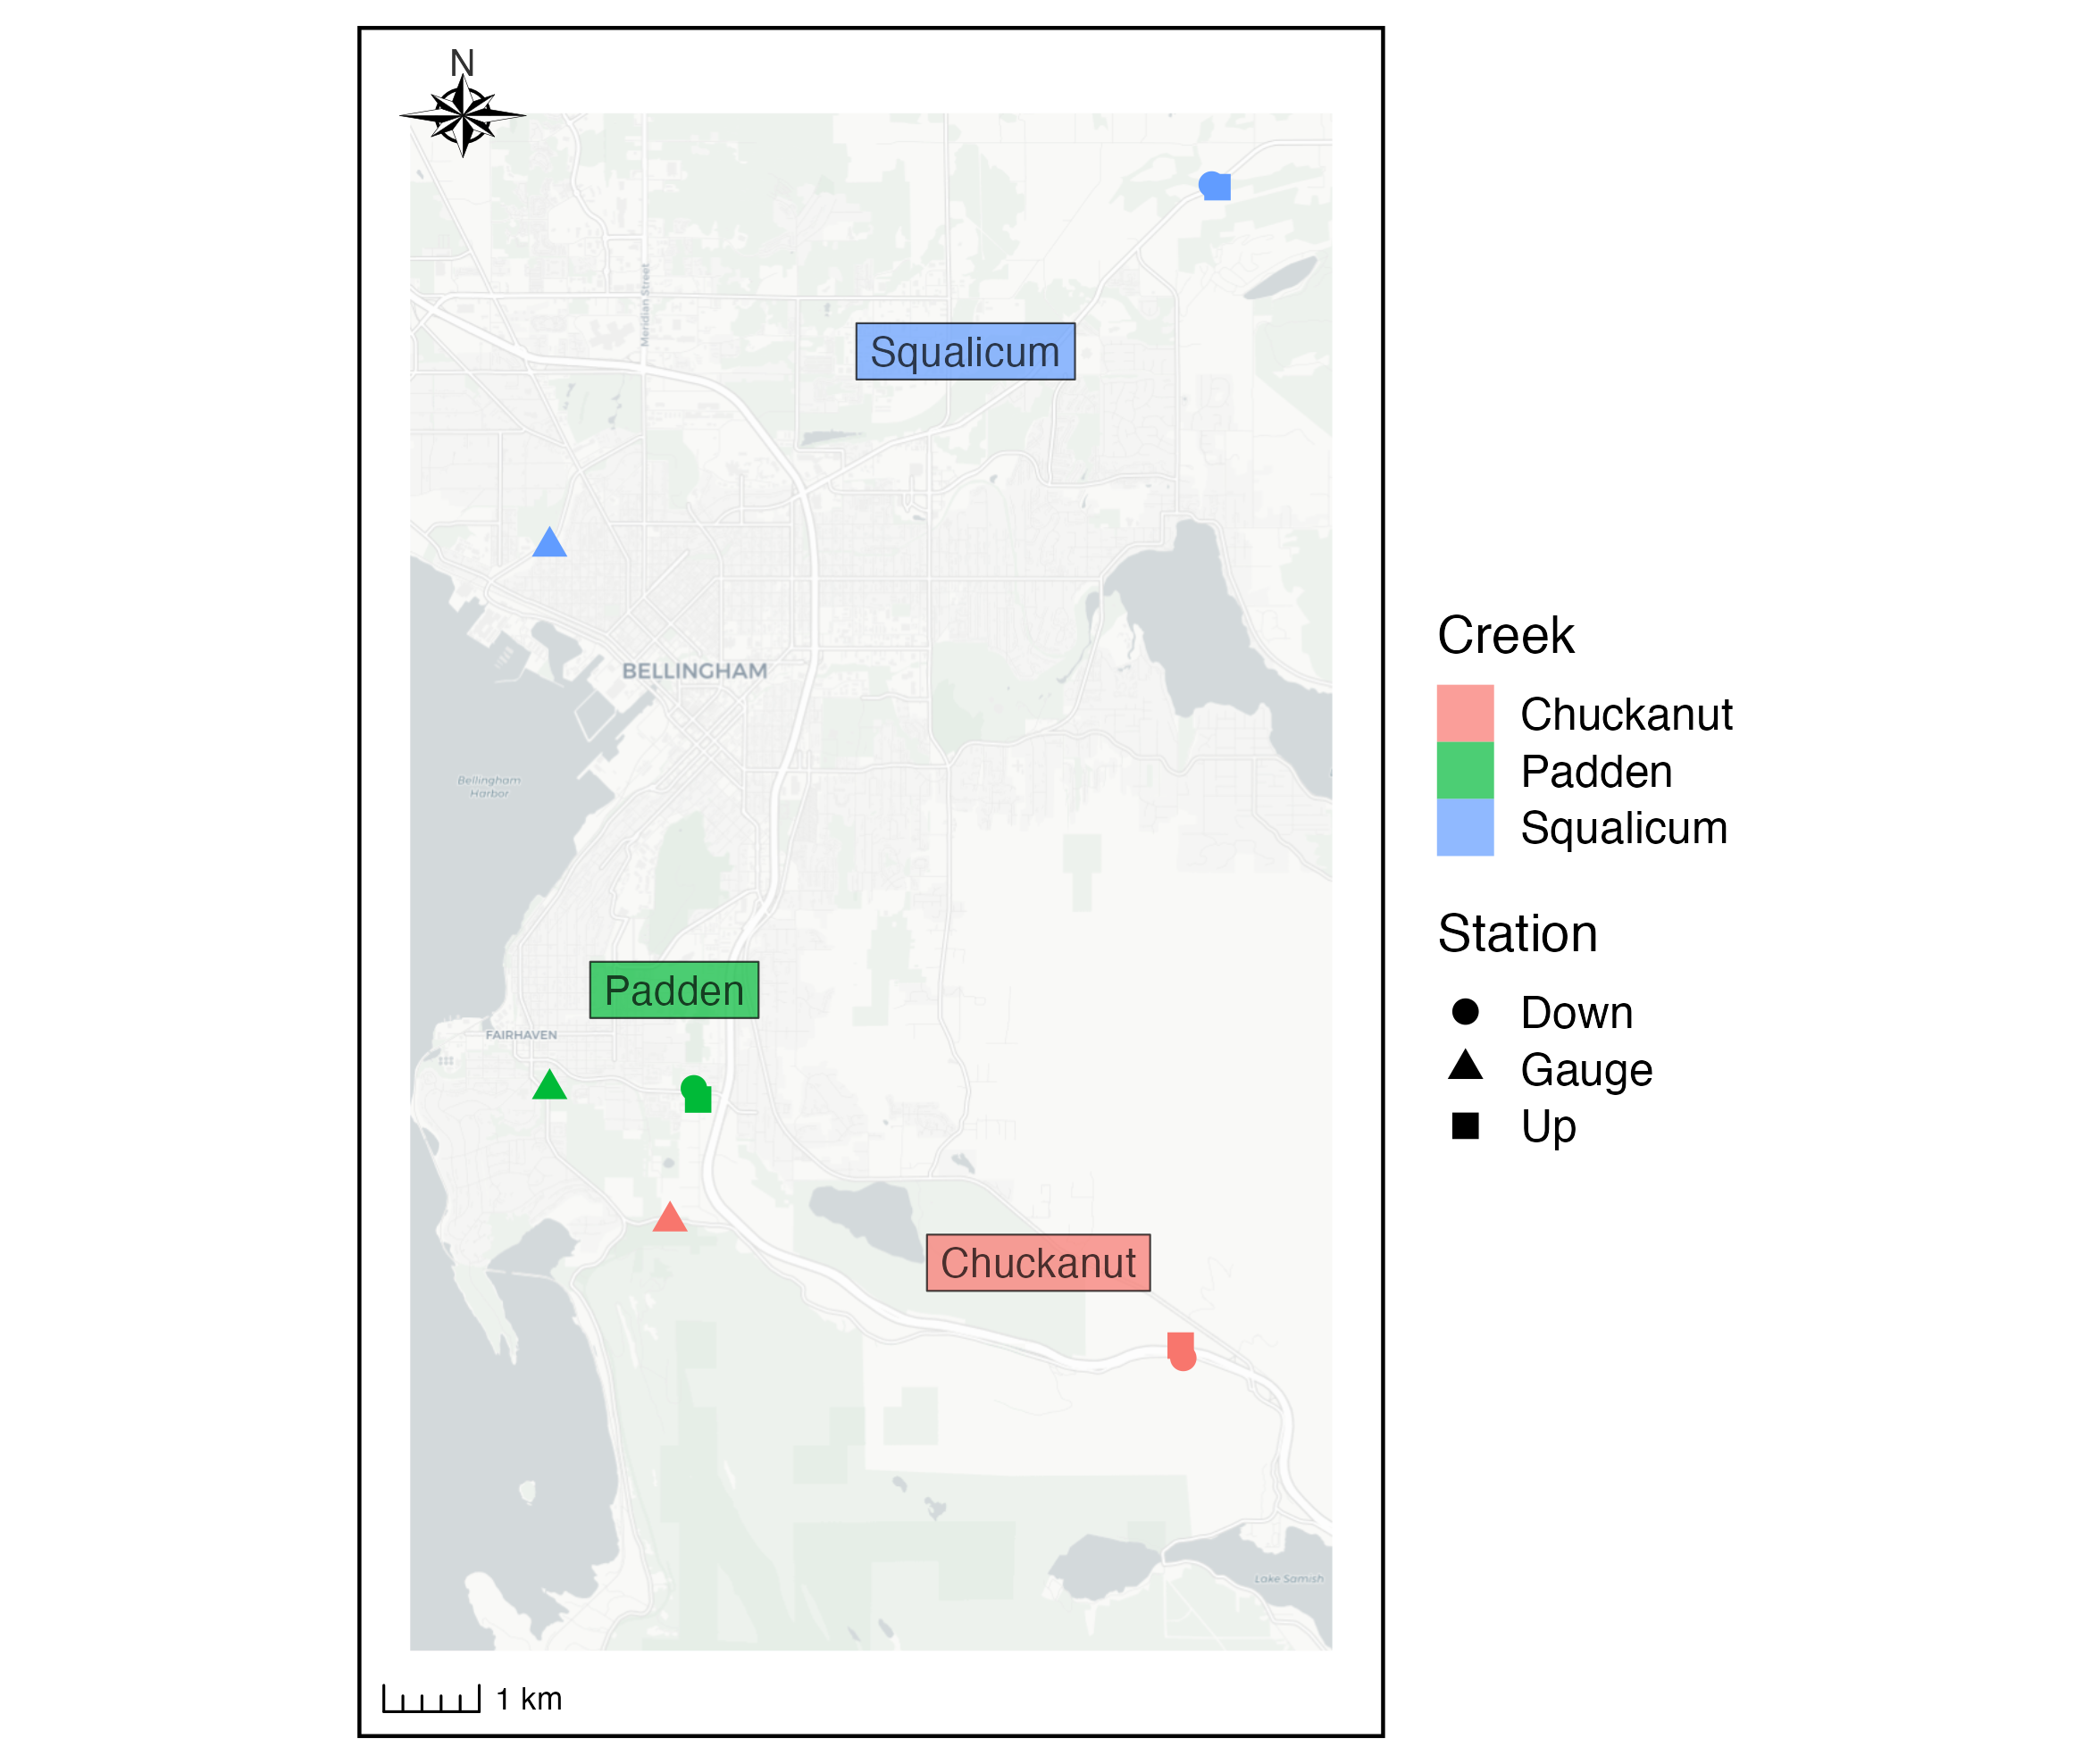
\includegraphics{../Output/SupplementalFigures/map_gauges.png}
\caption{Location of flow gauges compared to sampling locations for
Chuckanut, Padden, and Squalicum Creeks.}
\end{figure}

The flow meters at Squalicum Creek and Chuckanut Creek were offline from
November 2021 for the remainder of the sampling period. The highest
discharge seen during the course of the study from January to November
2021 occurred in November 2021 at Squalicum Creek. The mean discharge in
each creek was: 0.42 m\textsuperscript{3}/s in Padden, 0.29
m\textsuperscript{3}/s in Chuckanut, and 1.14 m\textsuperscript{3}/s in
Squalicum Creek. The lowest discharge registered by the flow meters is
0.0028 m\textsuperscript{3}/s, which occurred 8.5\%, 1.6\%, and 0.78\%
of the time in Padden, Chuckanut, and Squalicum, respectively.

Due to the lack of flow meter in Squalicum and Chuckanut Creeks from
November 2021 to February 2022, we used historical data from the three
flow gauges to calculate the average discharge for each day of the year
from about 2015-2021 (Supplementary Figure 2). We then used the value
for the day of the year that we sampled in either 2021 or 2022 when the
gauges were offline. For consistency, we also did this at Padden Creek
despite the gauge there being online for the entire sampling period.

\begin{figure}
\centering
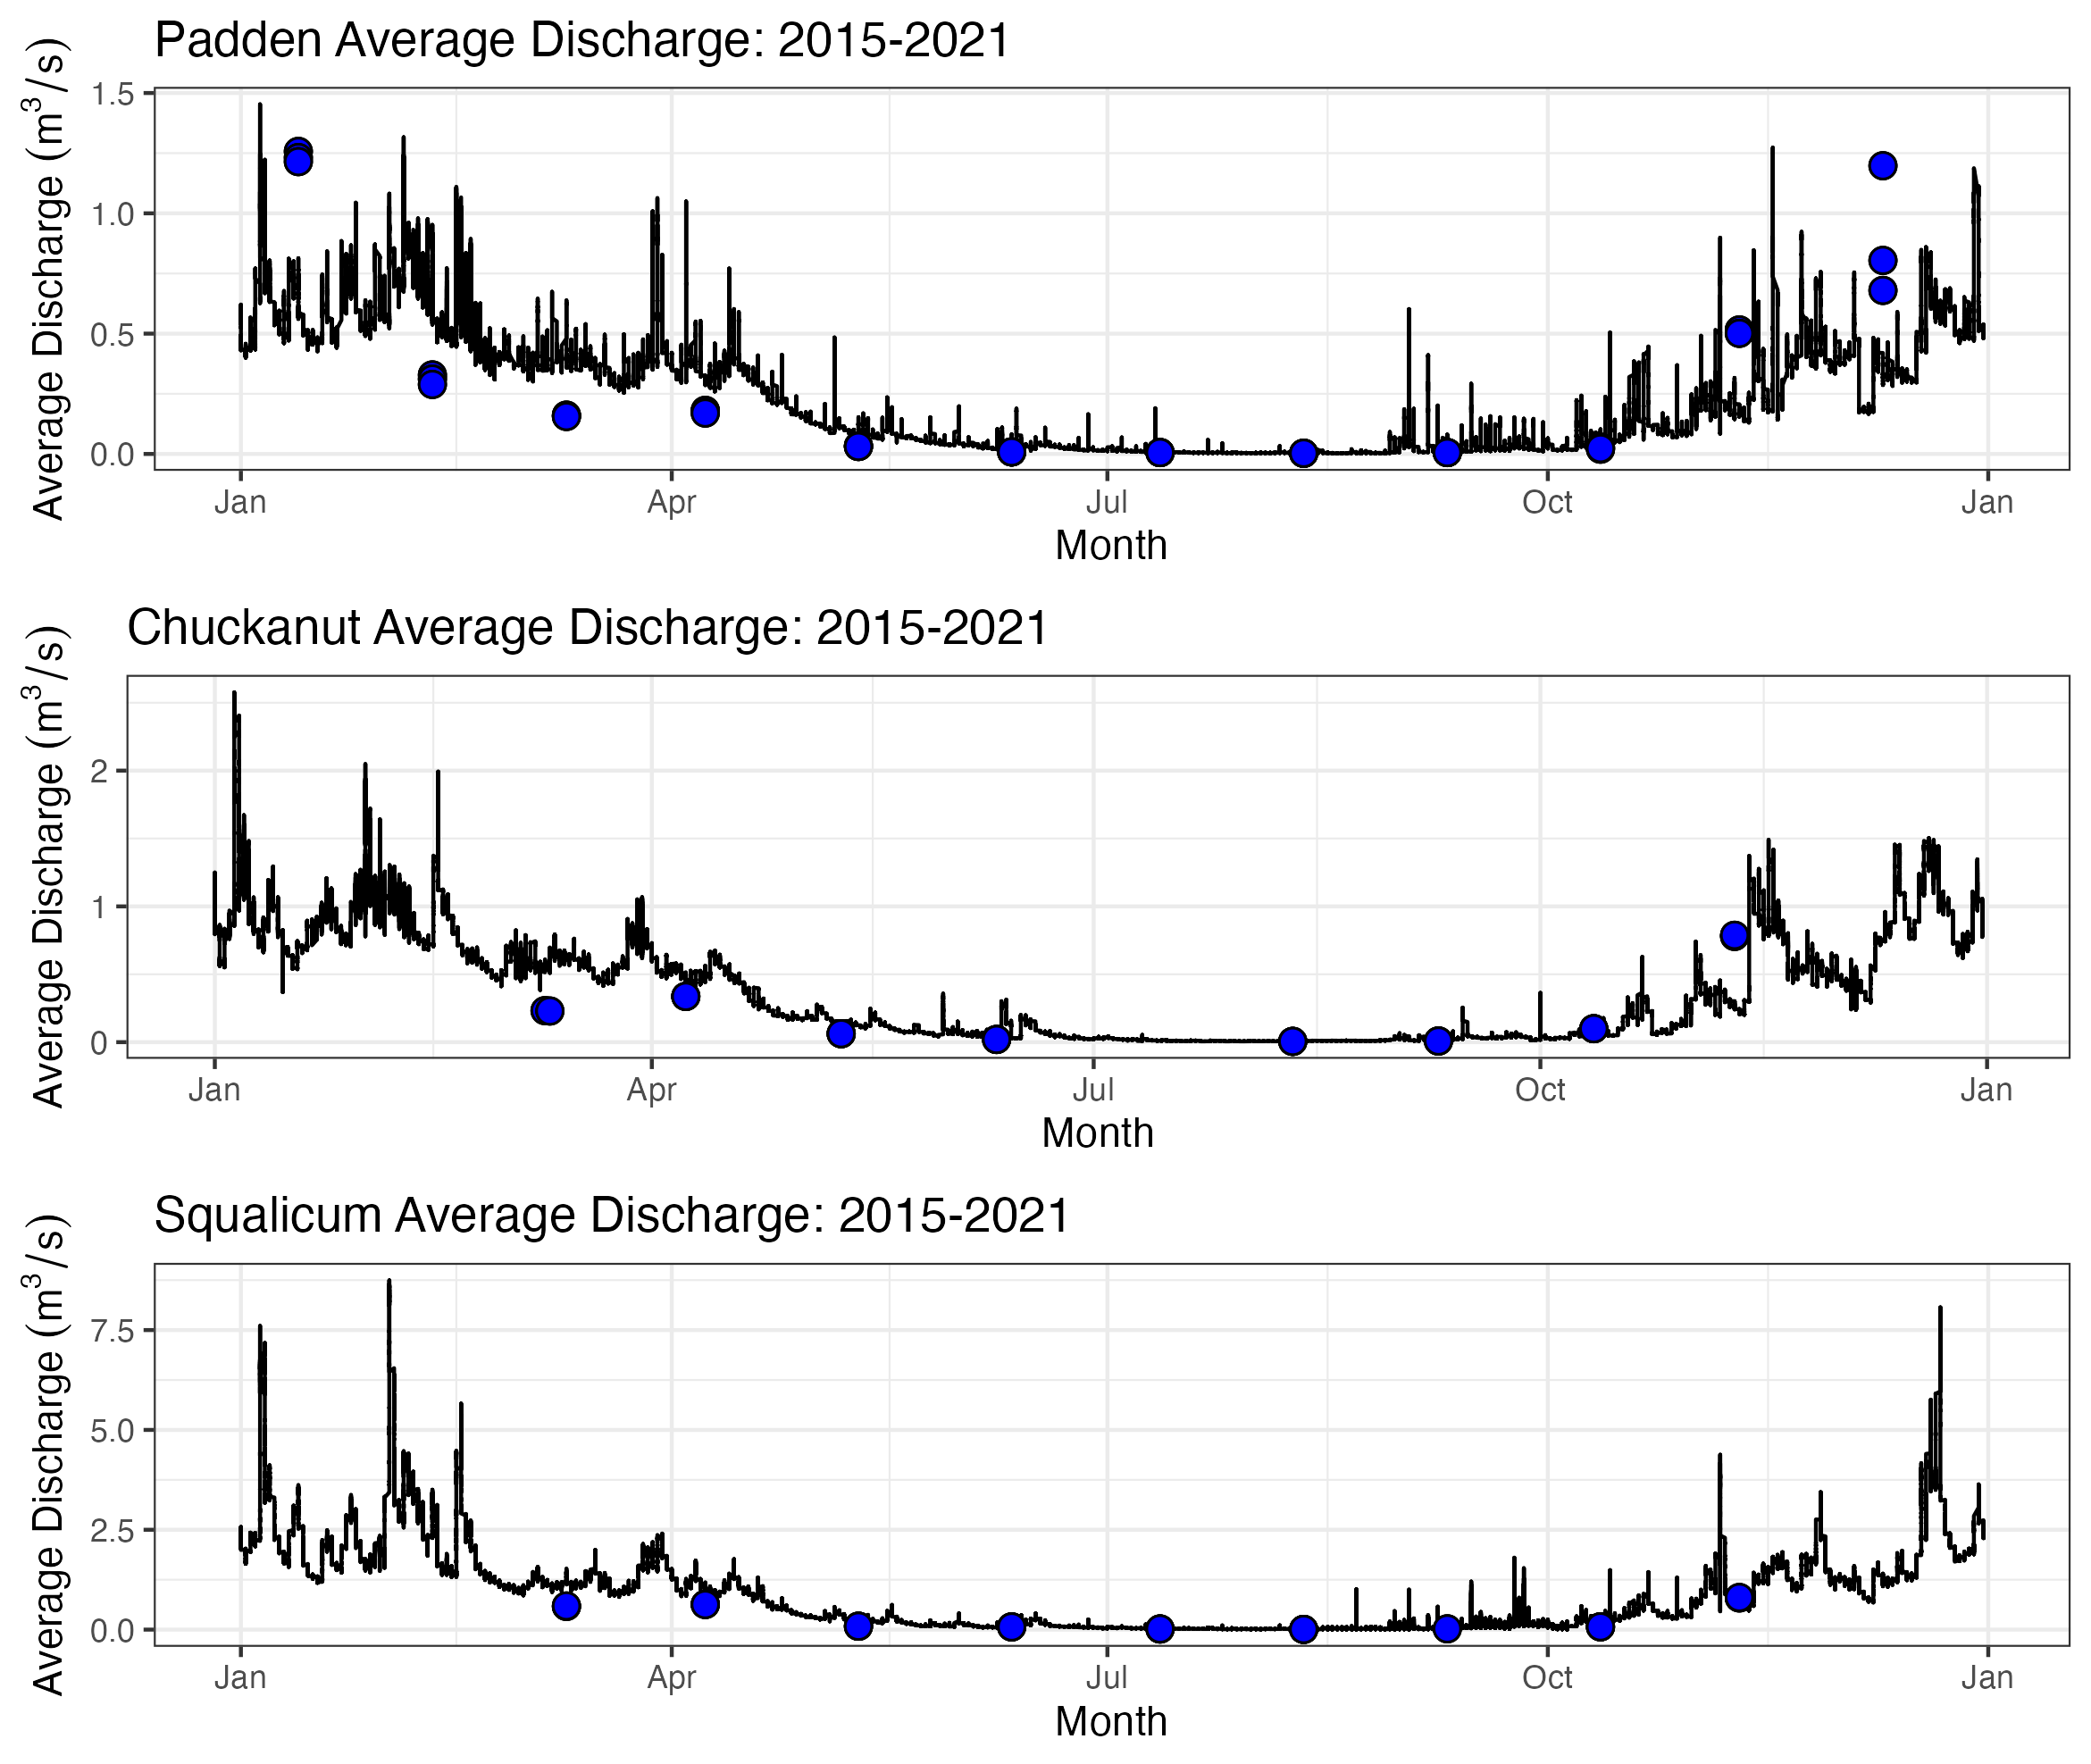
\includegraphics{../Output/SupplementalFigures/historical_flow_year_avg_sampling.png}
\caption{Discharge in creeks with USGS gauges. Note that Chuckanut and
Squalicum went offline around November 2021. Lines show the value for
each day averaged over 2015-2021. Blue dots show the time of sampling
during the course of this study.}
\end{figure}

\hypertarget{stocking-in-lake-padden}{%
\subsubsection{Stocking in Lake Padden}\label{stocking-in-lake-padden}}

Padden Lake has historically been stocked with hatchery fish by the
Washington Department of Fish and Wildlife (Supplementary Figure 3).
During the course of the study, a total of 10,000 rainbow trout were
stocked in April and May 2021, 30,000 kokanee salmon were stocked in May
2021, and 10,000 cutthroat trout were stocked in January 2021 two months
before sampling began in March. However, Lake Padden is 1.5 km upstream
of the sampling locations in Padden Creek and we do not expect to see an
increased signal due to the flow from the lake after stocking events.

\begin{figure}
\centering
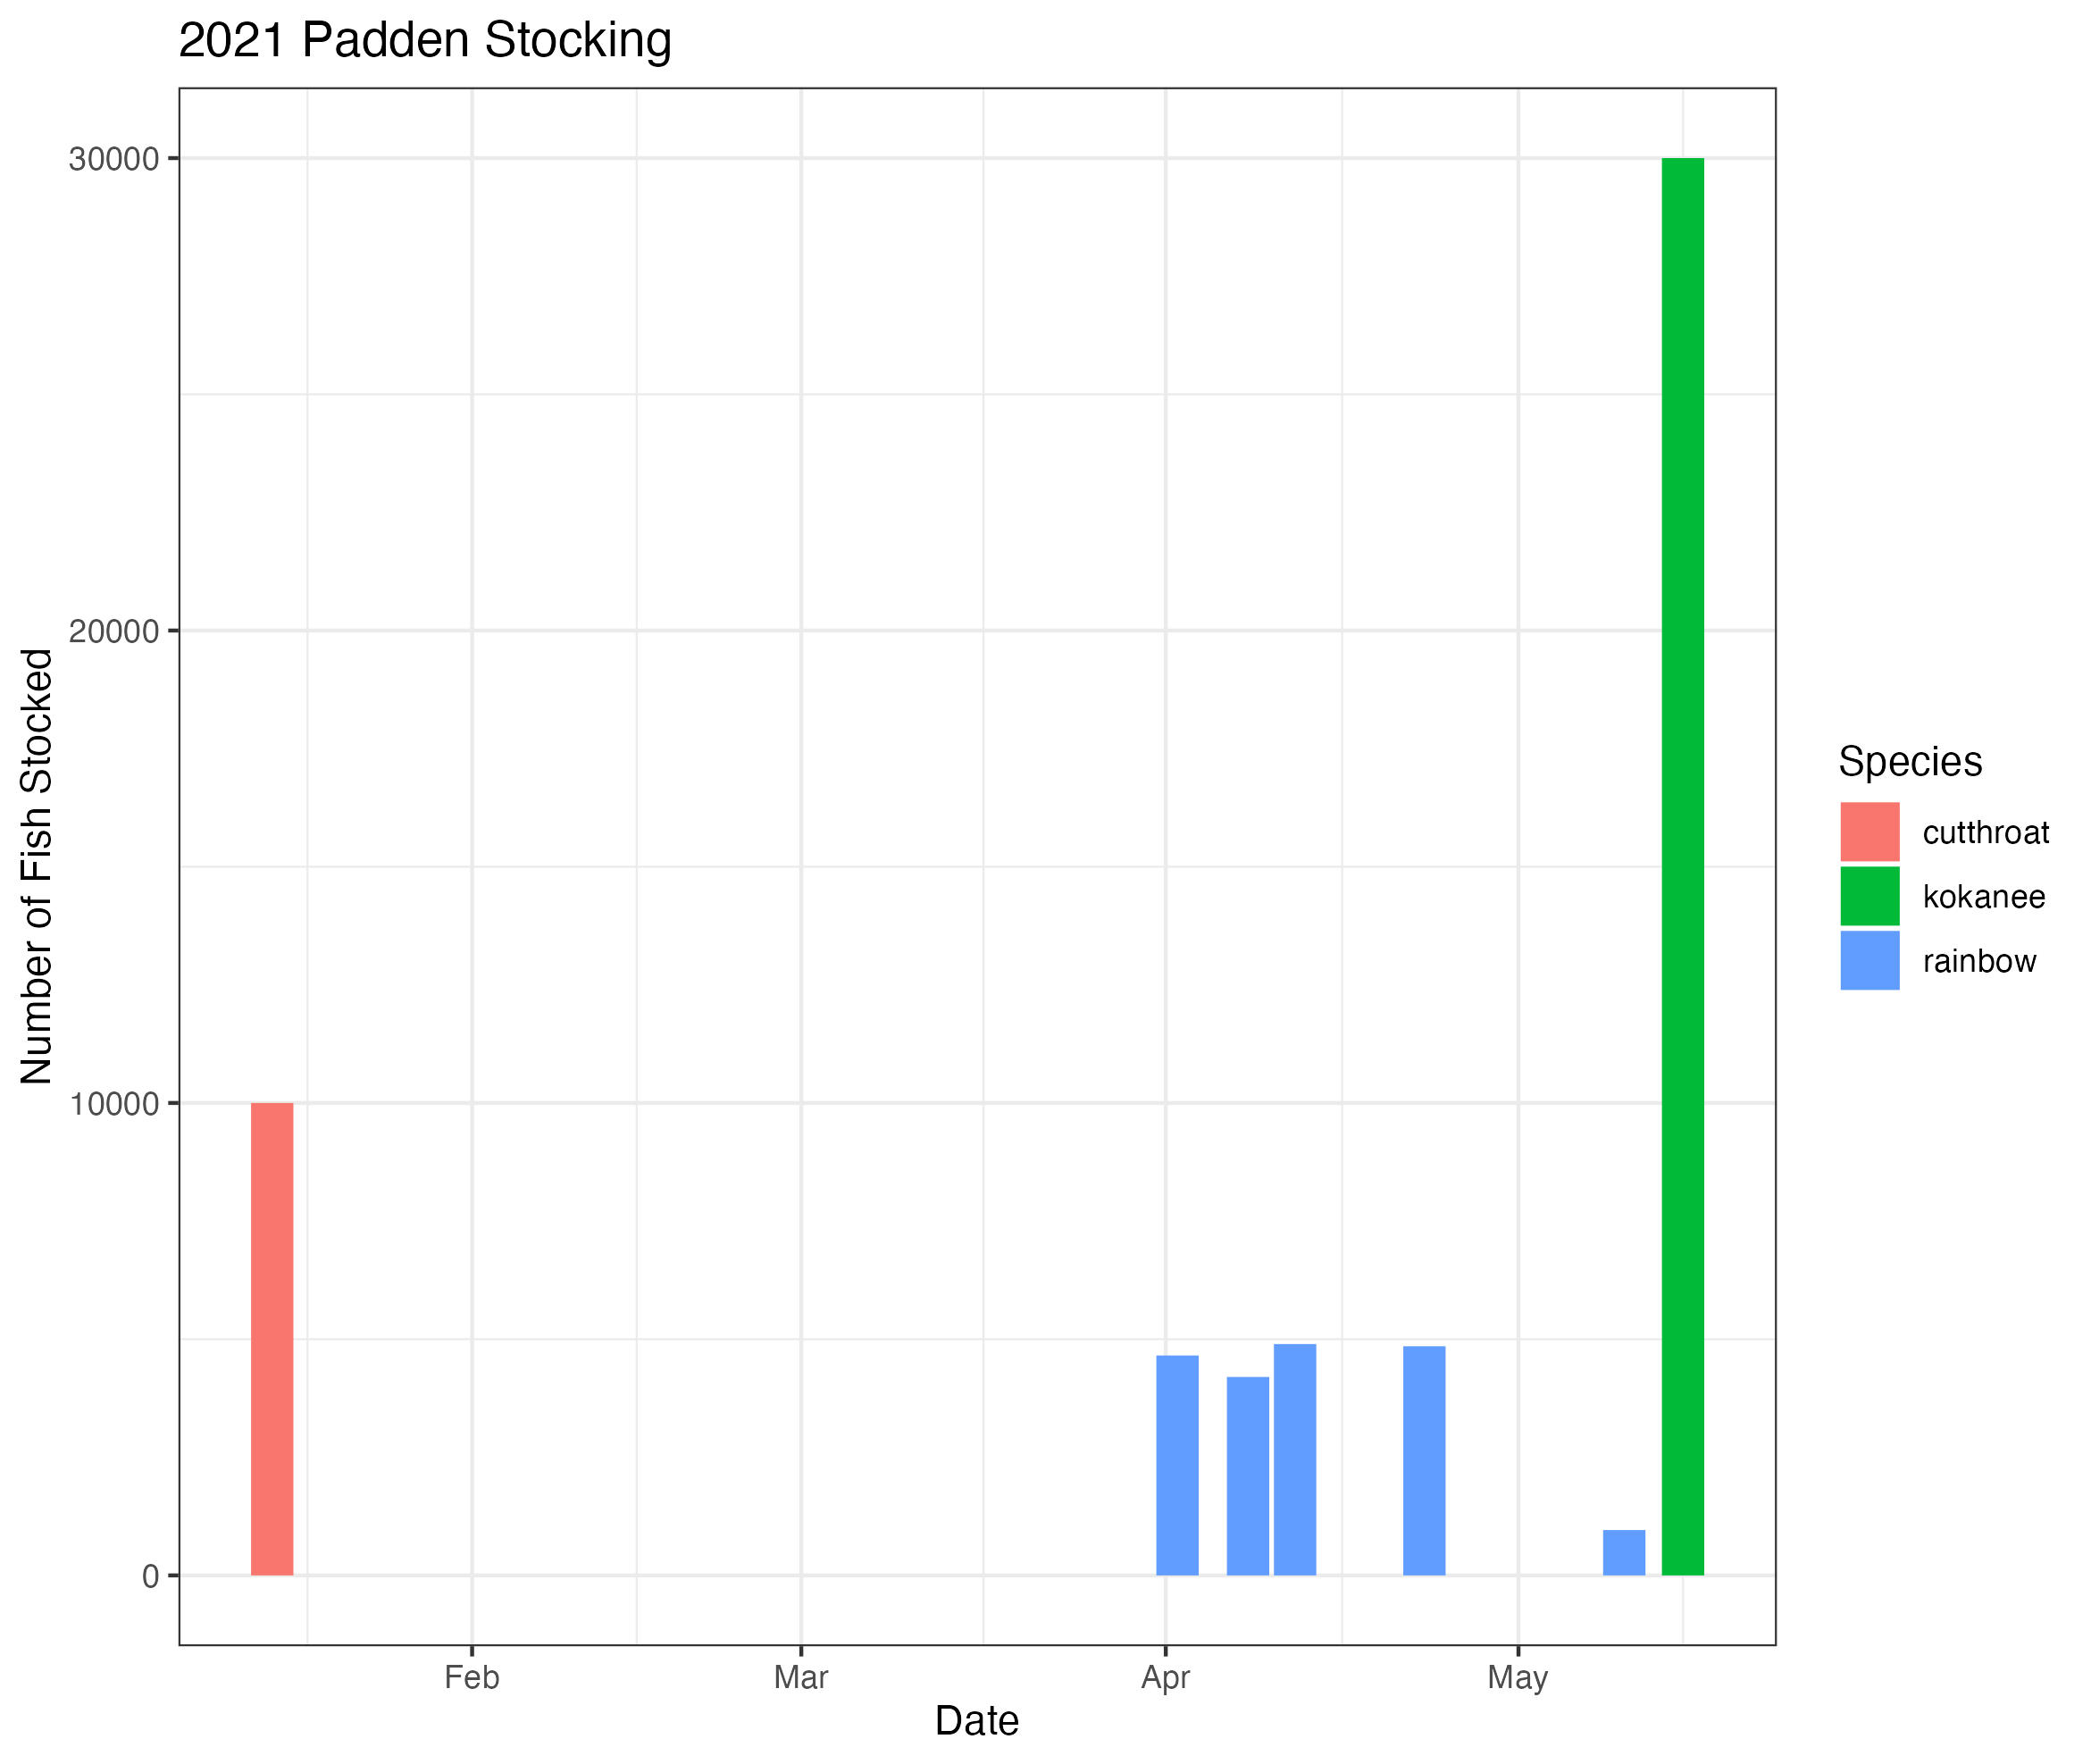
\includegraphics{../Output/SupplementalFigures/stocking_2021only.png}
\caption{Stocking of Lake Padden in 2021.}
\end{figure}

\hypertarget{water-sampling}{%
\subsubsection{Water Sampling}\label{water-sampling}}

Water samples were collected using Smith Root's eDNA Backpack (Austen C.
Thomas et al. 2018), a portable pumping-and-filtering setup set to
filter at 1 L/min at 82.7 kPa (12 psi). For most months, a trident
sampler was used to collect all 3 biological replicates at the exact
same time, for a total sampling time of about 5 minutes. Otherwise, the
three replicates were collected consecutively, for a total sampling time
of about 15 minutes. The backpack also monitored pressure and flow rate
over the course of sampling. The backpack was set to have a target flow
rate of 1 L/min and a max pressure of 12 psi. Downstream sites were
always sampled before upstream sites to ensure no potential DNA was
introduced into the stream before sampling. In some months, less than 2
L of water was filtered due to clogging (Supplemental Figure 4).

\begin{figure}
\centering
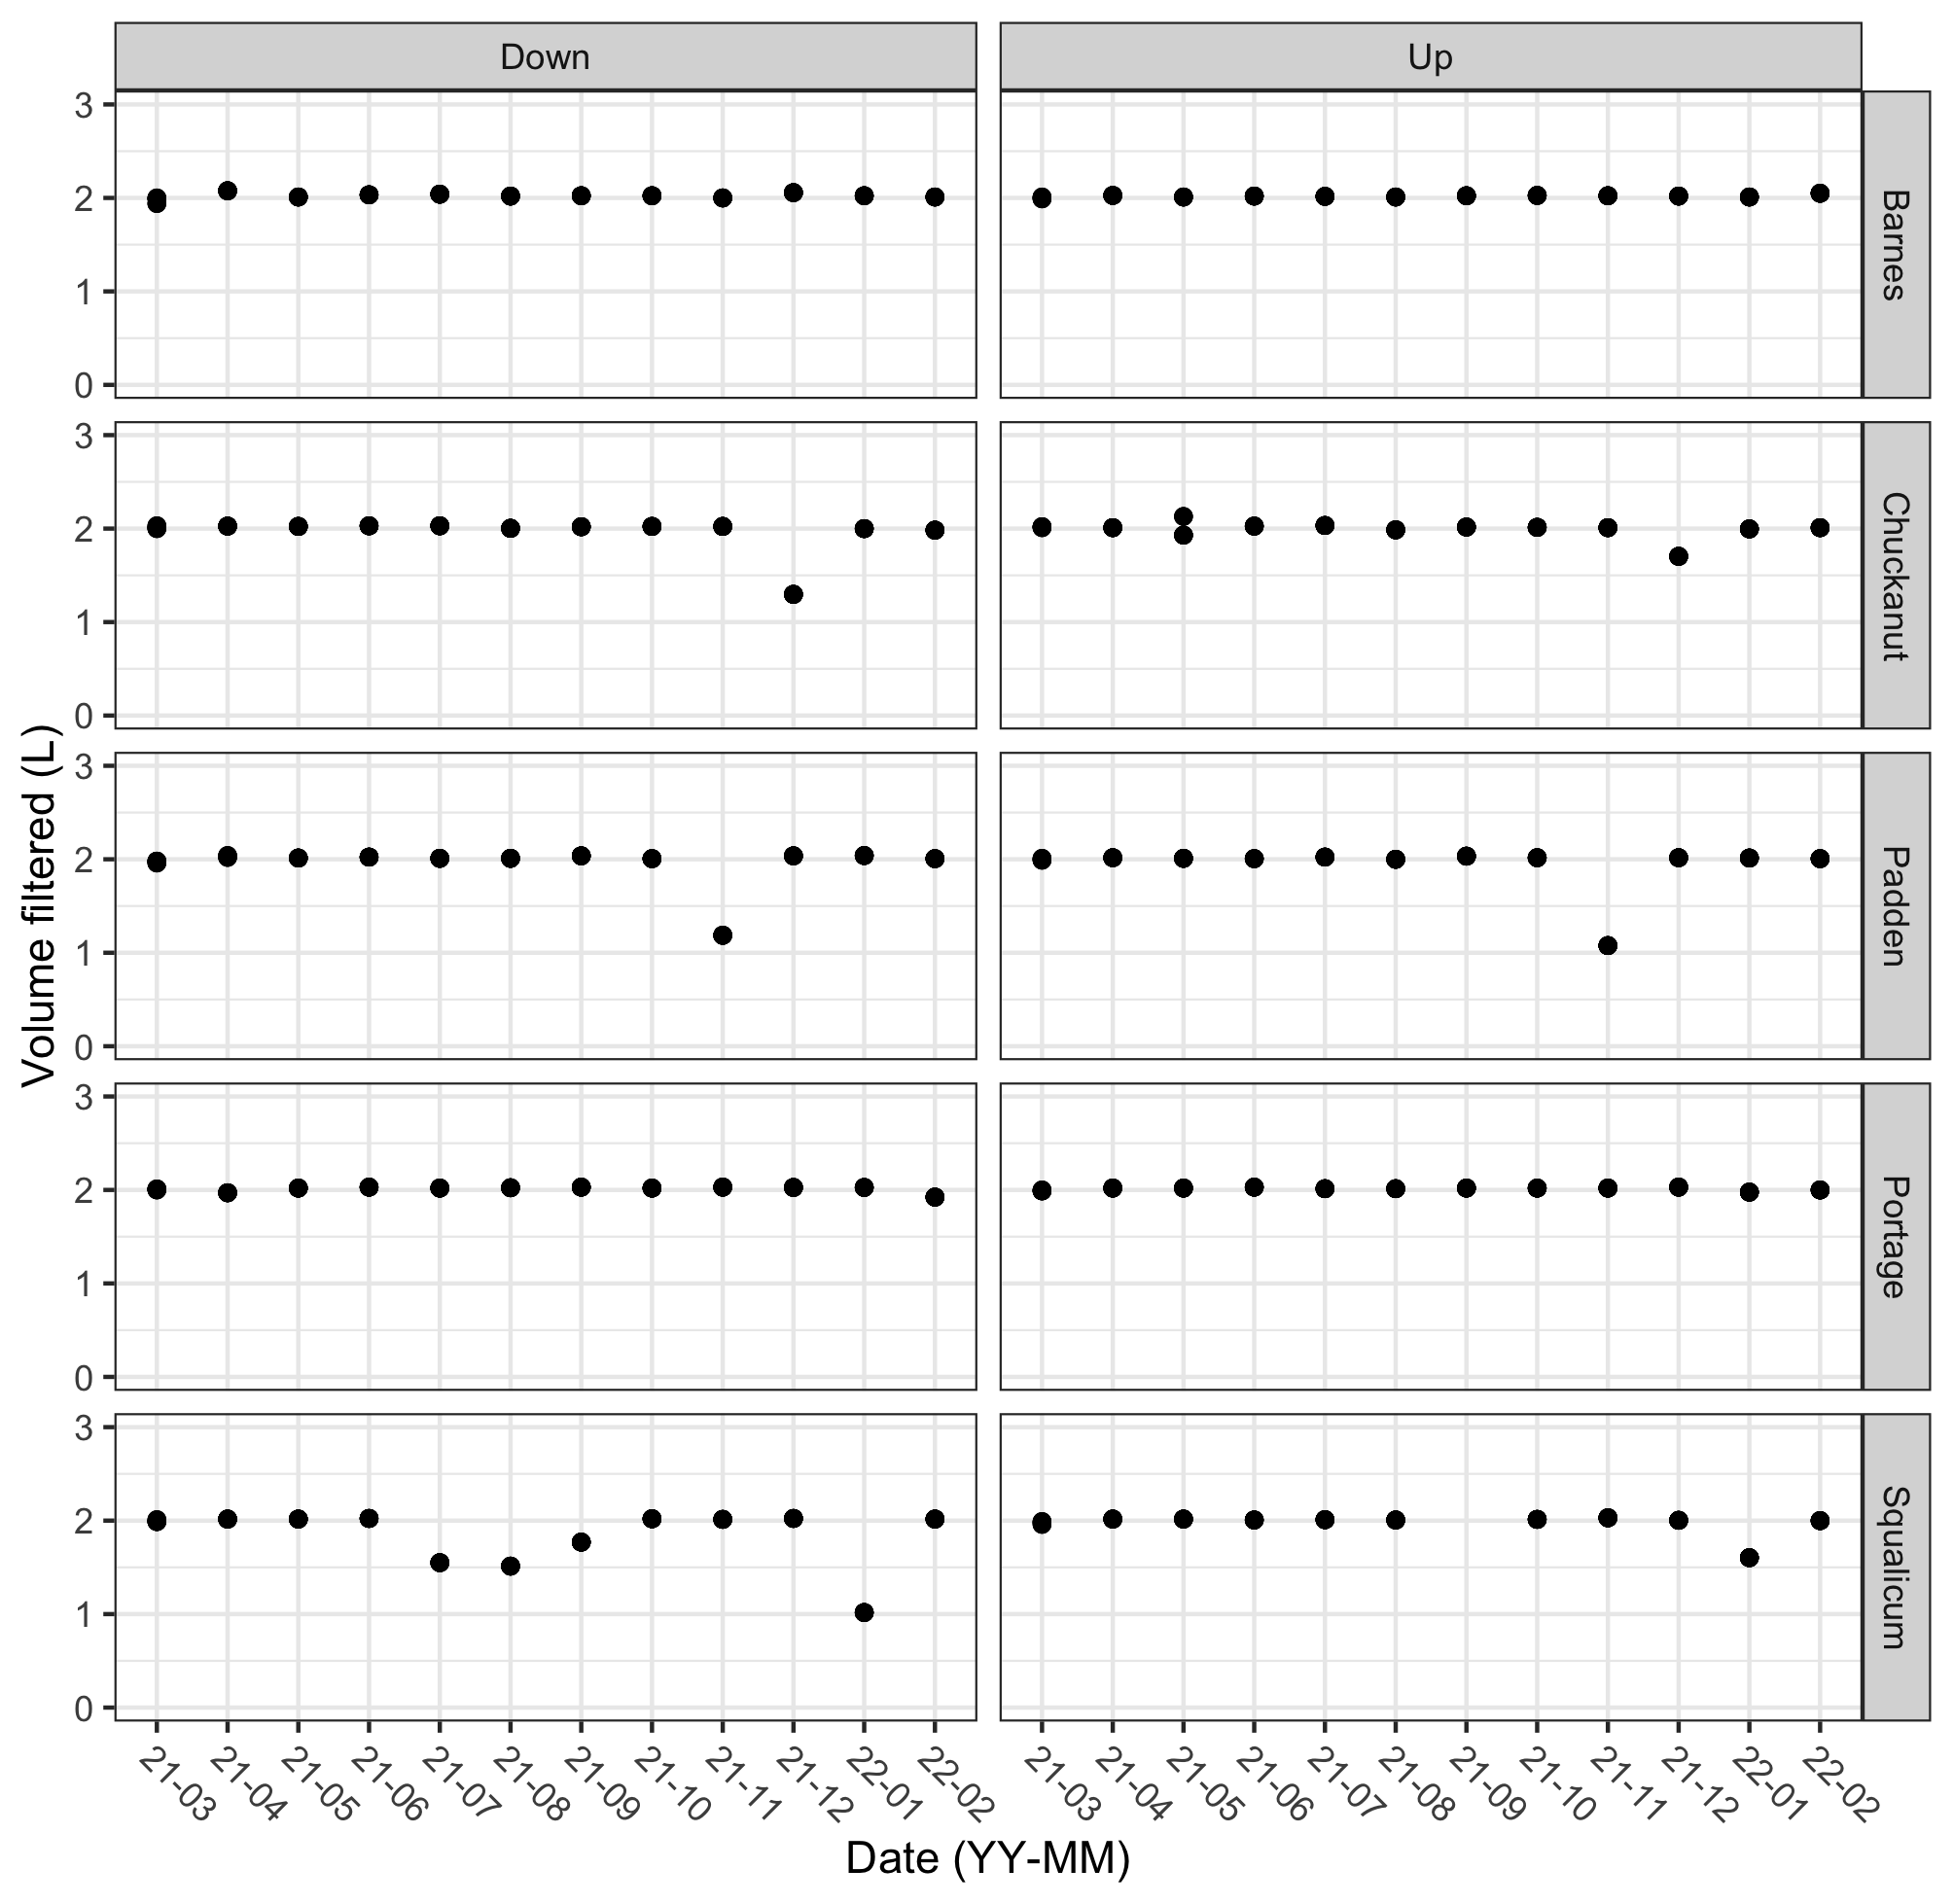
\includegraphics{../Output/SupplementalFigures/volume_filtered_by_sample.png}
\caption{Volume filtered (L) for each sample. Note that Squalicum
upstream in September 2021 was completely dry and therefore no water was
filtered.}
\end{figure}

\hypertarget{laboratory-processing}{%
\subsection{Laboratory Processing}\label{laboratory-processing}}

\hypertarget{dna-extractions}{%
\subsubsection{DNA Extractions}\label{dna-extractions}}

We followed a protocol developed for extracting DNA off the
self-preserving Smith Root filters (Austen C. Thomas et al. 2019).
Filters were removed from their housing with sterile tweezers and cut in
half using sterile razor blades. One half was archived and the other
half was used for extraction. The extraction was performed using the
Qiagen DNeasy Blood and Tissue Kit (Qiagen, USA) with minor
modifications, including adding a Qiashredder column (Qiagen, USA).

\hypertarget{pcr-amplification}{%
\subsubsection{PCR Amplification}\label{pcr-amplification}}

PCR reactions included 10 \(\mu\)L of 5X Platinum ii Buffer, 0.4
\(\mu\)L of Platinum ii Taq, 1.25 \(\mu\)L of 8 mM dNTPS, 1.25 \(\mu\)L
of 10 \(\mu\)M F primer, 1.25 \(\mu\)L of 10 \(\mu\)M R primer, 5
\(\mu\)L of template, and 30.85 \(\mu\)L of molecular grade water, for a
total reaction volume of 50 \(\mu\)L. Cycling conditions were as
follows: 95\degree C for 2 min, 35 cycles of 95\degree C for 30 sec,
60\degree C for 30 sec, 72\degree C for 30 sec, followed by a final
extension of 72\degree C for 5 min.

For indexing, 10 ng of PCR product was used as template in a final
volume of 11.25 \(\mu\)L For samples with concentrations less than 0.88
ng/\(\mu\)L, 11.25 \(\mu\)L was added despite being less than 10 ng of
amplicon. Each sample received a unique index; Nextera index sets A and
B were used in combination to avoid using the same index for more than
one sample on a single sequencing run. The PCR reaction included the
11.25 \(\mu\)L of template, 12.5 \(\mu\)L of Kapa HiFi MMX (Roche, USA),
and 1.25 \(\mu\)L of indexed primer. Cycling conditions were as follows:
95\degree C for 5 min, 8 cycles of 98\degree C for 20 sec, 56\degree C
for 30 sec, 72\degree C for 3 min, and a final extension of 72\degree C
for 5 min.

\hypertarget{species-specific-qpcr}{%
\subsubsection{Species Specific qPCR}\label{species-specific-qpcr}}

Each DNA sample was run in triplicate using Gene Expression Mastermix
(ThermoFisher, USA), a final concentration of 0.375 \(\mu\)M F primer,
0.375 \(\mu\)M R primer, and 0.105 \(\mu\)M probe, as well as 1X EXO-IPC
mix, 1X EXO-IPC DNA, 3.5 \(\mu\)L of template for a final reaction
volume of 12 \(\mu\)L. The EXO-IPC mix includes the primers and probe
for the EXI-IPC DNA, with the probe having a VIC reporter, allowing it
to be multiplexed with the \emph{O. clarkii} assay, which has a FAM
reporter.

Thermocycling was as follows: 50\degree C for 2 min, 95\degree C for 10
min, followed by 45 cycles of 95\degree C for 15 sec, 60\degree C for 1
min. The cycle threshold (Ct) value determined for the EXO-IPC assay
from the NTC was compared to the Ct value for the EXO-IPC assay in each
of the environmental samples. If the Ct value was \textgreater0.5 Ct
values from the mean Ct for the NTCs, the sample was deemed inhibited
and diluted 1:10 and re-assayed until the Ct value fell within the
accepted range (Supplementary Figure 5). After converting Ct values to
DNA concentrations using the standard curve (see below), the
concentration was multiplied by the dilution factor.

\begin{figure}
\centering
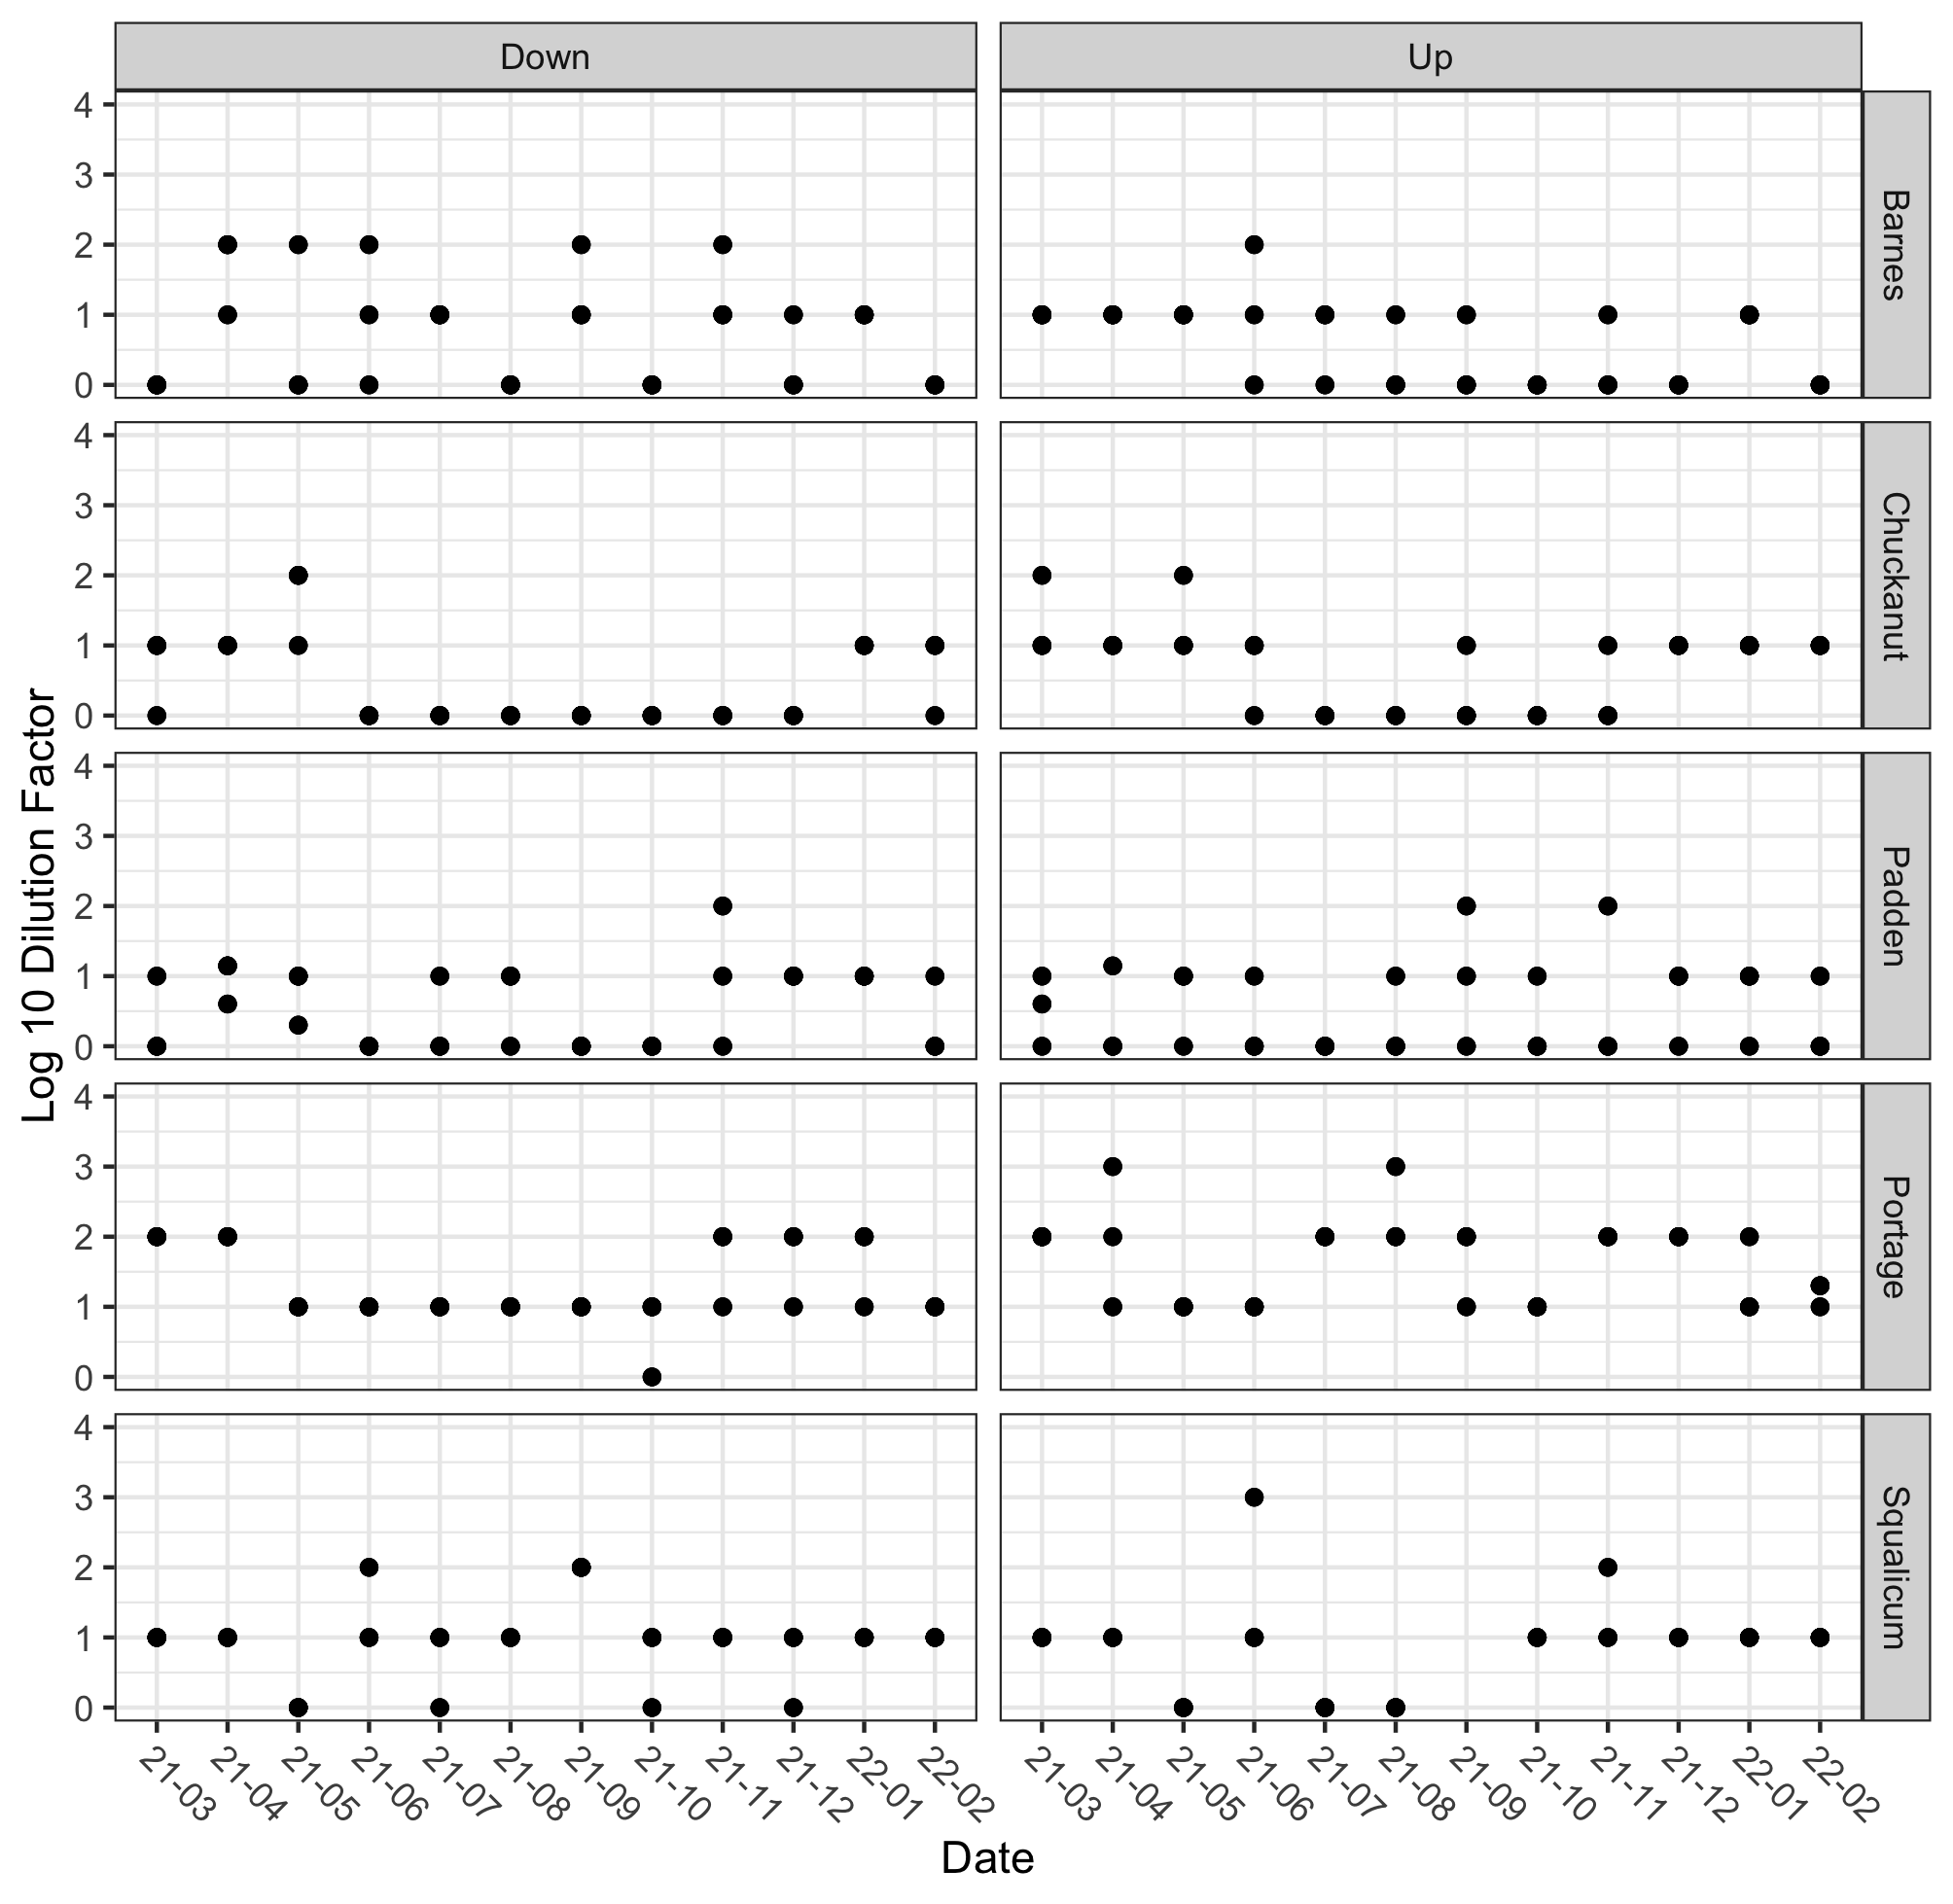
\includegraphics{../Output/SupplementalFigures/inhibition_dilution_factors.png}
\caption{Dilution factor required to remove inhibition as measured by an
internal positive control (IPC) qPCR assay.}
\end{figure}

\hypertarget{bioinformatics-processing}{%
\subsection{Bioinformatics Processing}\label{bioinformatics-processing}}

Primers were removed with cutadapt (Martin 2011) and then reads were
de-noised, filtered, merged, and ASVs were generated using dada2
(Callahan et al. 2016). For each MiSeq run, the trimming lengths were
determined by visually assessing the quality score plots. After ASVs
were generated, taxonomy was assigned using the ``classify'' function in
the insect package in R using the classifier published by the authors of
the package (Wilkinson et al. 2018).

\hypertarget{quality-controls}{%
\subsubsection{Quality Controls}\label{quality-controls}}

Positive controls were included on each sequencing run to monitor for
cross contamination that might have occurred in the laboratory or due to
``tag jumping''. With 13 MiSeq runs, we included one sample of kangaroo
tissue on each run and then measured how many reads of kangaroo were
found in environmental samples and how many reads of non-kangaroo were
found in kangaroo samples (Supplementary Figure 6).

\begin{figure}
\centering
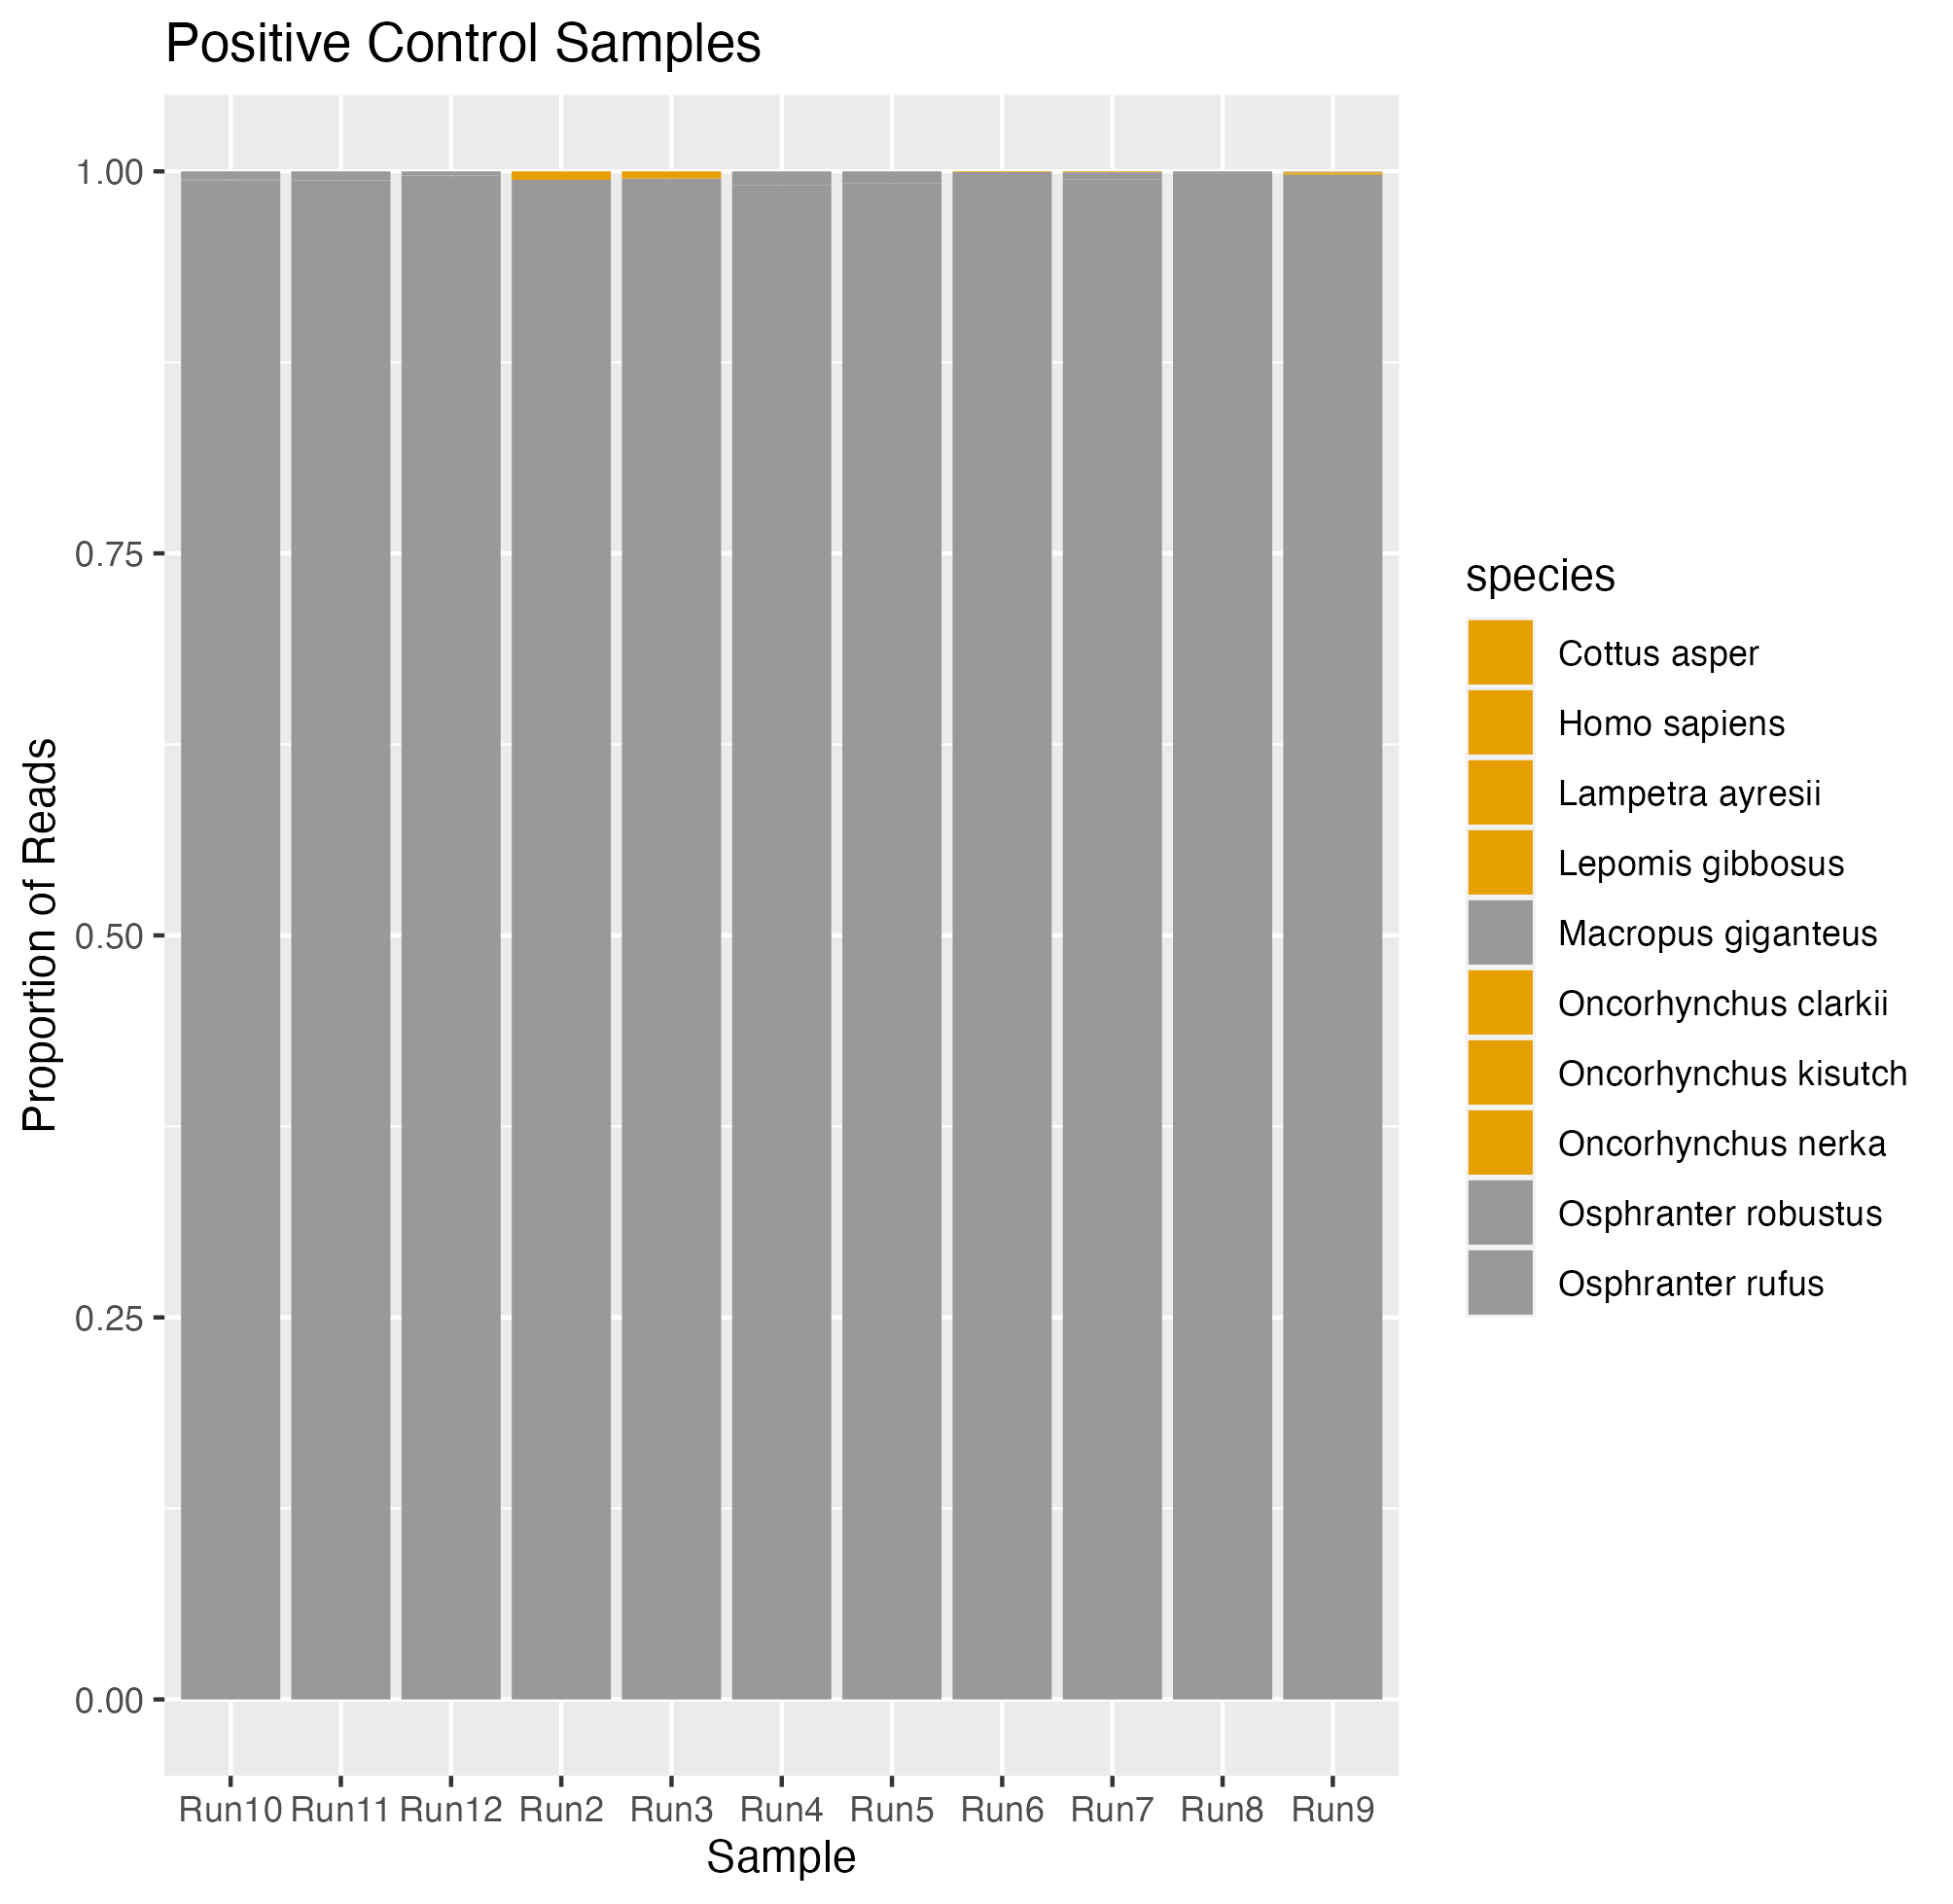
\includegraphics{../Output/SupplementalFigures/check_controls.png}
\caption{Proporiton of annotated reads found in positive controls. Grey
colors are the three species of kangaroo used for positive controls and
are what should be in each sample. Orange species should not be in the
positive controls and indicate low level contamination from
environmental samples.}
\end{figure}

We can also check to make sure that no reads assigning to kangaroo were
in the environmental samples. We processed X environmental samples and
only 2 had any reads assigned to kangaroo (Supplementary Figure 7).

\begin{figure}
\centering
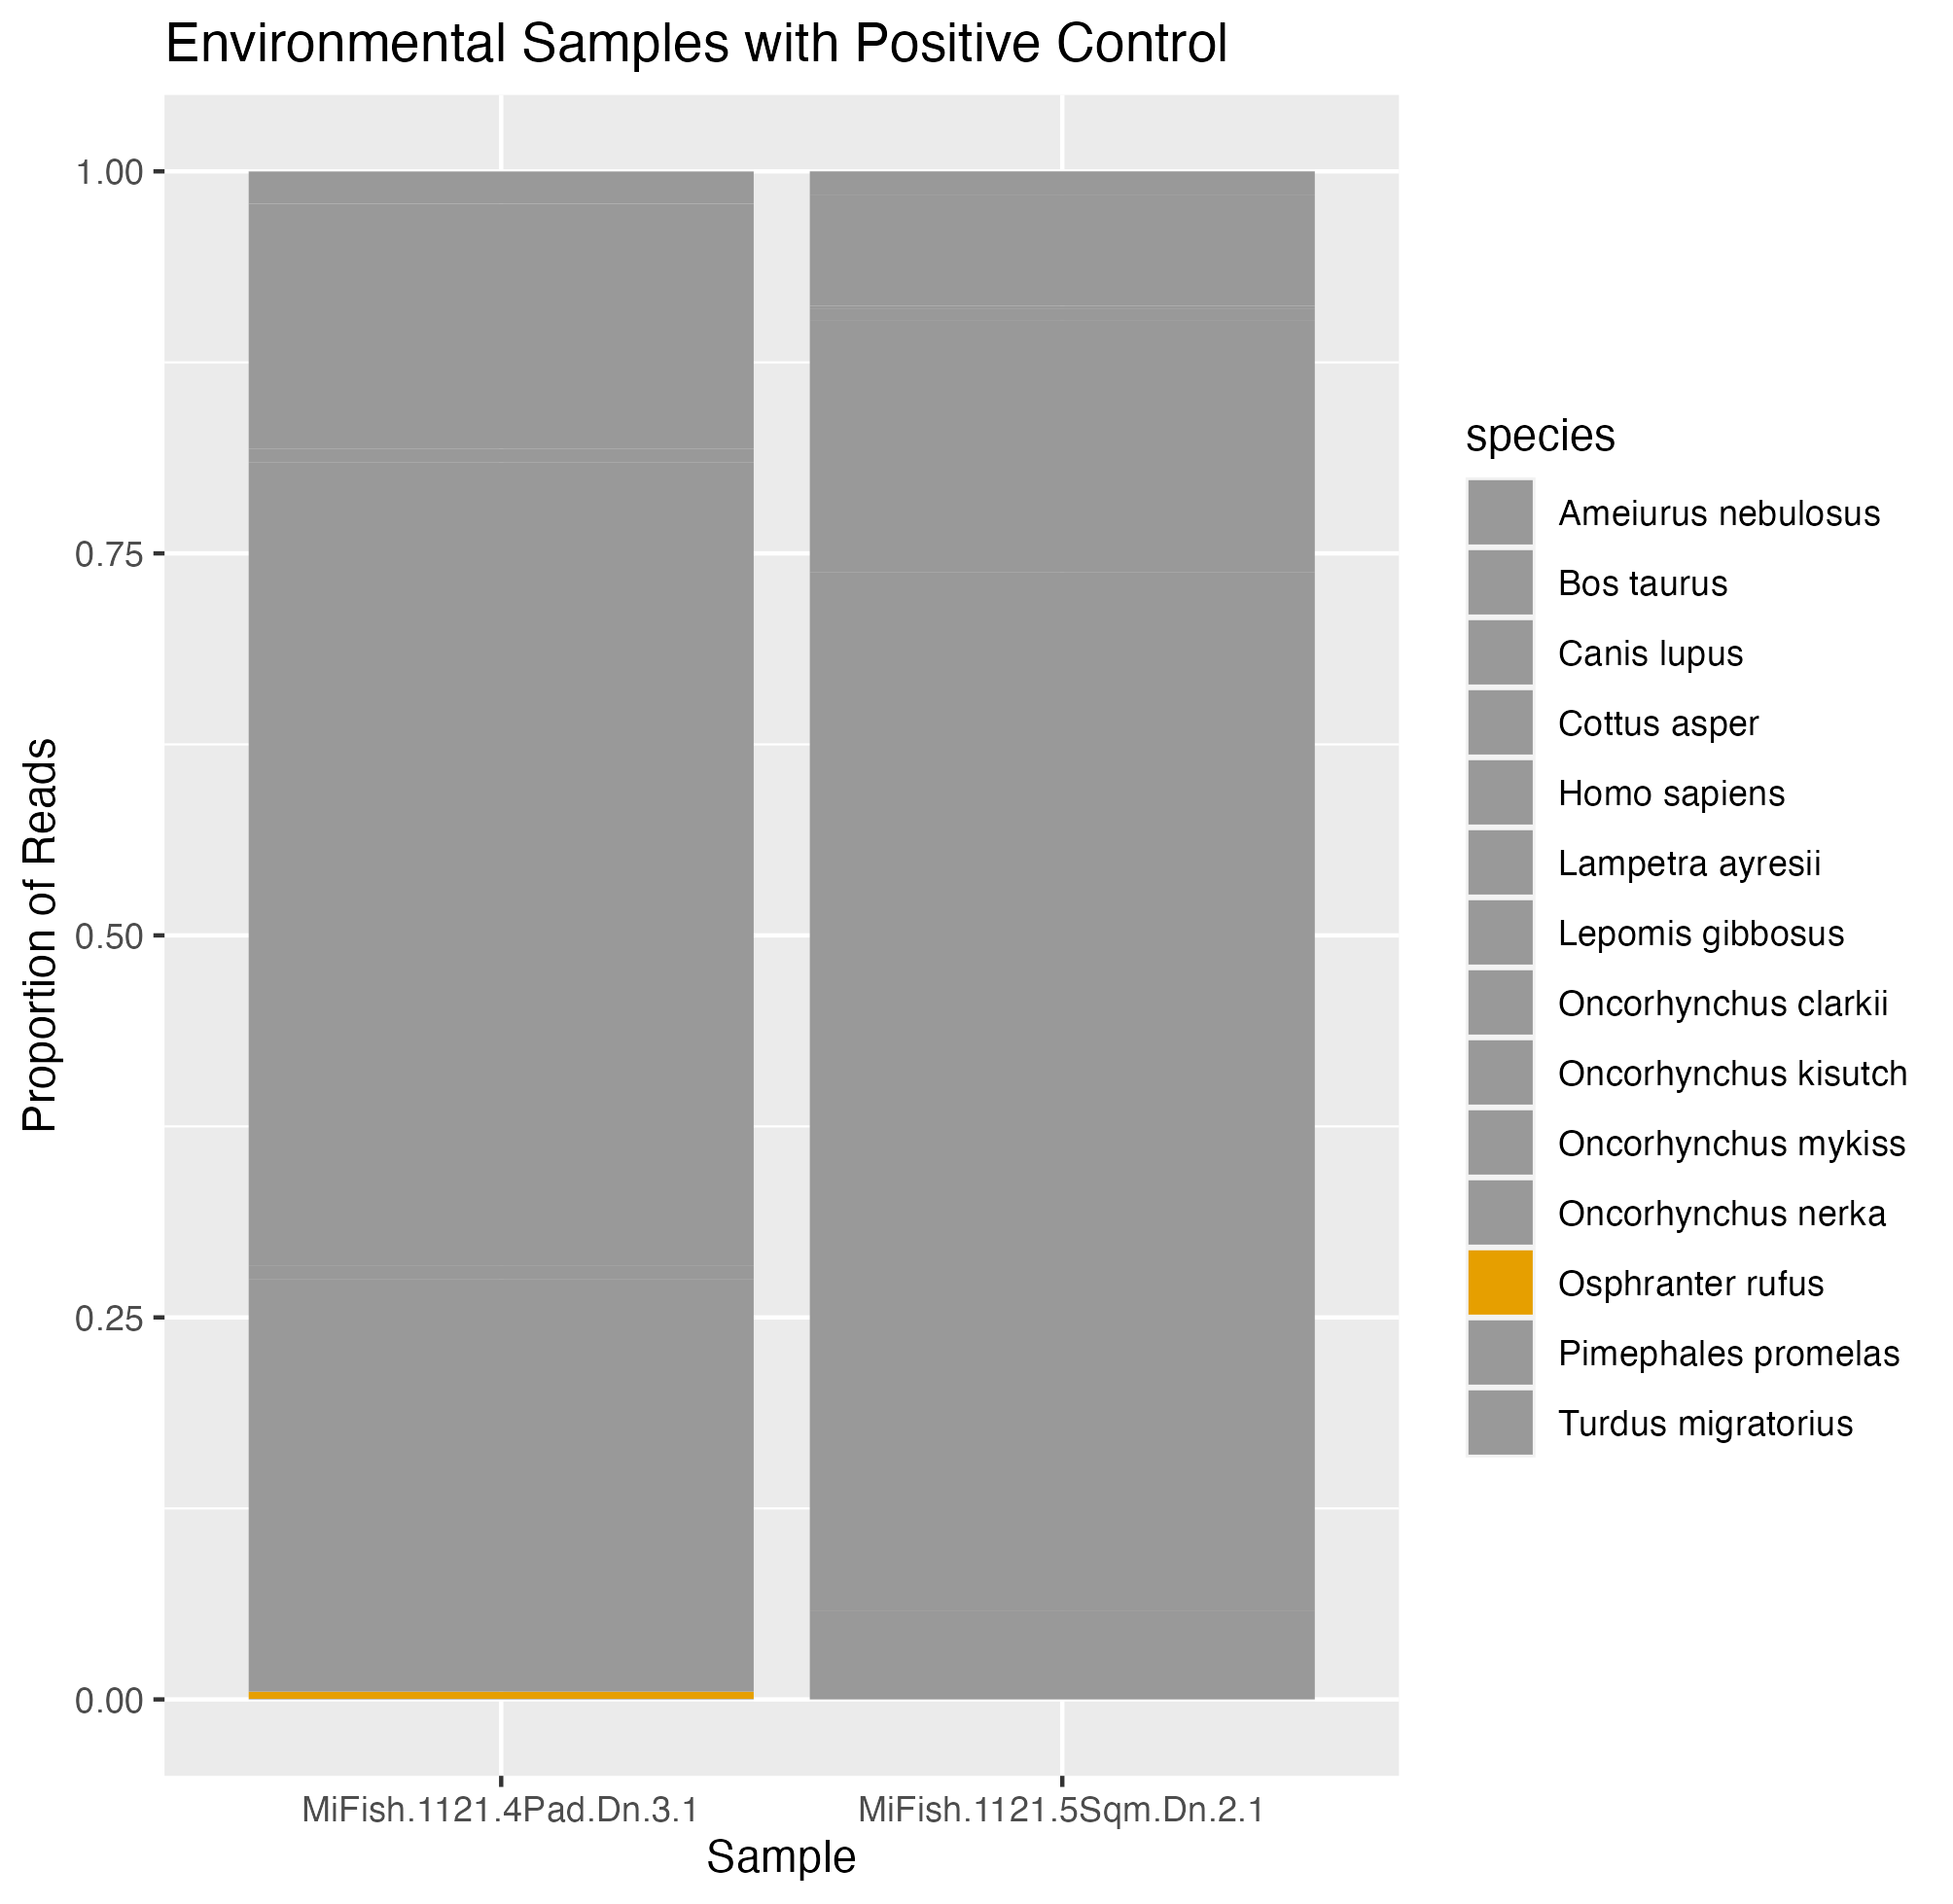
\includegraphics{../Output/SupplementalFigures/check_controls2.png}
\caption{Proporiton of annotated reads found in environmental samples
with positive control. Grey colors are non-kangaroo reads and therefore
and are what should be in each sample. Orange species are kangaroo reads
and therefore should not be in the environmental samples and indicate
low level contamination from positive controls.}
\end{figure}

\hypertarget{annotation}{%
\subsubsection{Annotation}\label{annotation}}

We first used a tree-based annotation method (insect package) and then
followed up with a BLAST search for all ASVs that were not annotated to
species level by insect.

\hypertarget{correcting-metabarcoding-data-for-amplification-bias}{%
\subsection{Correcting metabarcoding data for amplification
bias}\label{correcting-metabarcoding-data-for-amplification-bias}}

Using our six mock communities (three different taxa compositions x two
proportions {[}even and skewed{]}), we can first check how well the
quantitative metabarcoding model corrects for amplification bias. In one
case, we consider the even mock communities as the mock community data
and the skewed mock communities as unknown. We can then re-create what
the model believes to be the original starting proportions of the skewed
mock community given the proportions of reads found in the skewed mock
communities and the proportion of DNA as compared to the proportion of
reads found in the even mock communities. We can also do the same
treating the skewed mock communities as known and even mock communities
as unknown (Supplementary Figure 7).

\begin{figure}
\centering
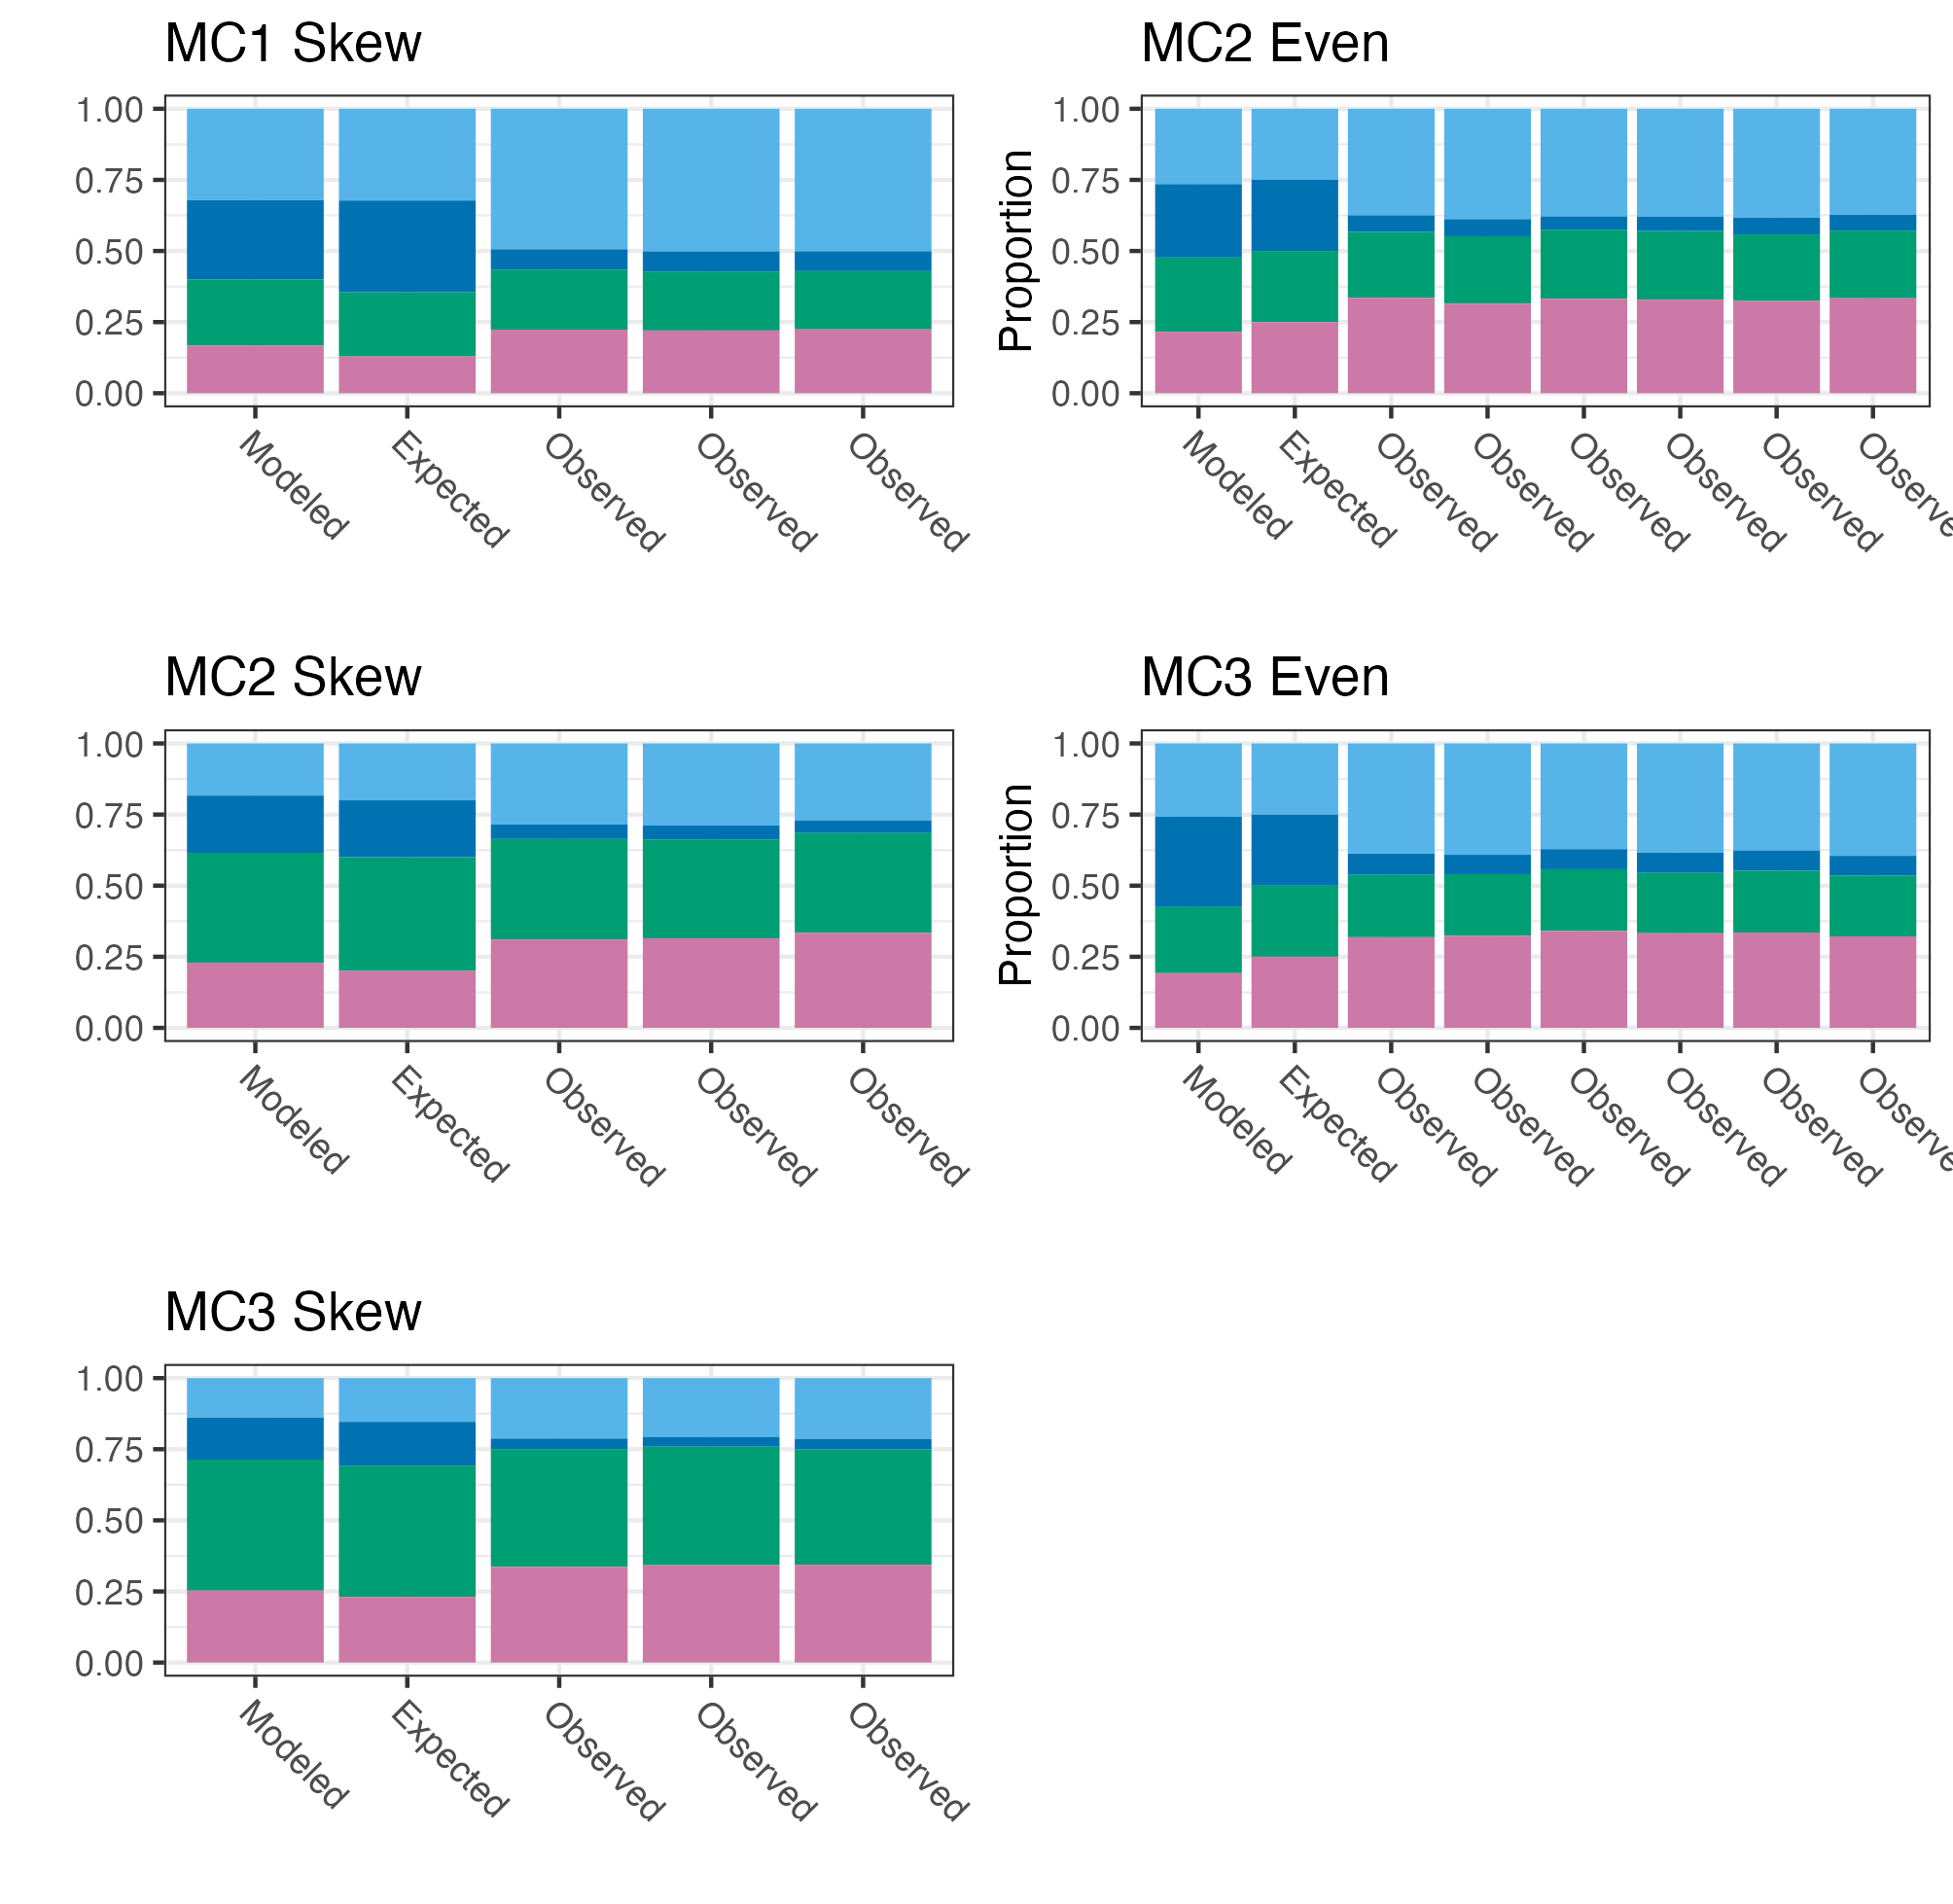
\includegraphics{../Output/SupplementalFigures/mock_internal_calibration.png}
\caption{Intercalibration of mock communities used to correct
environmental samples for amplification bias.}
\end{figure}

We can also check how well the calibration is working by comparing the
alpha values by using different subsets of mock community data as true
and unknown (Supplementary Figure 8).

\begin{figure}
\centering
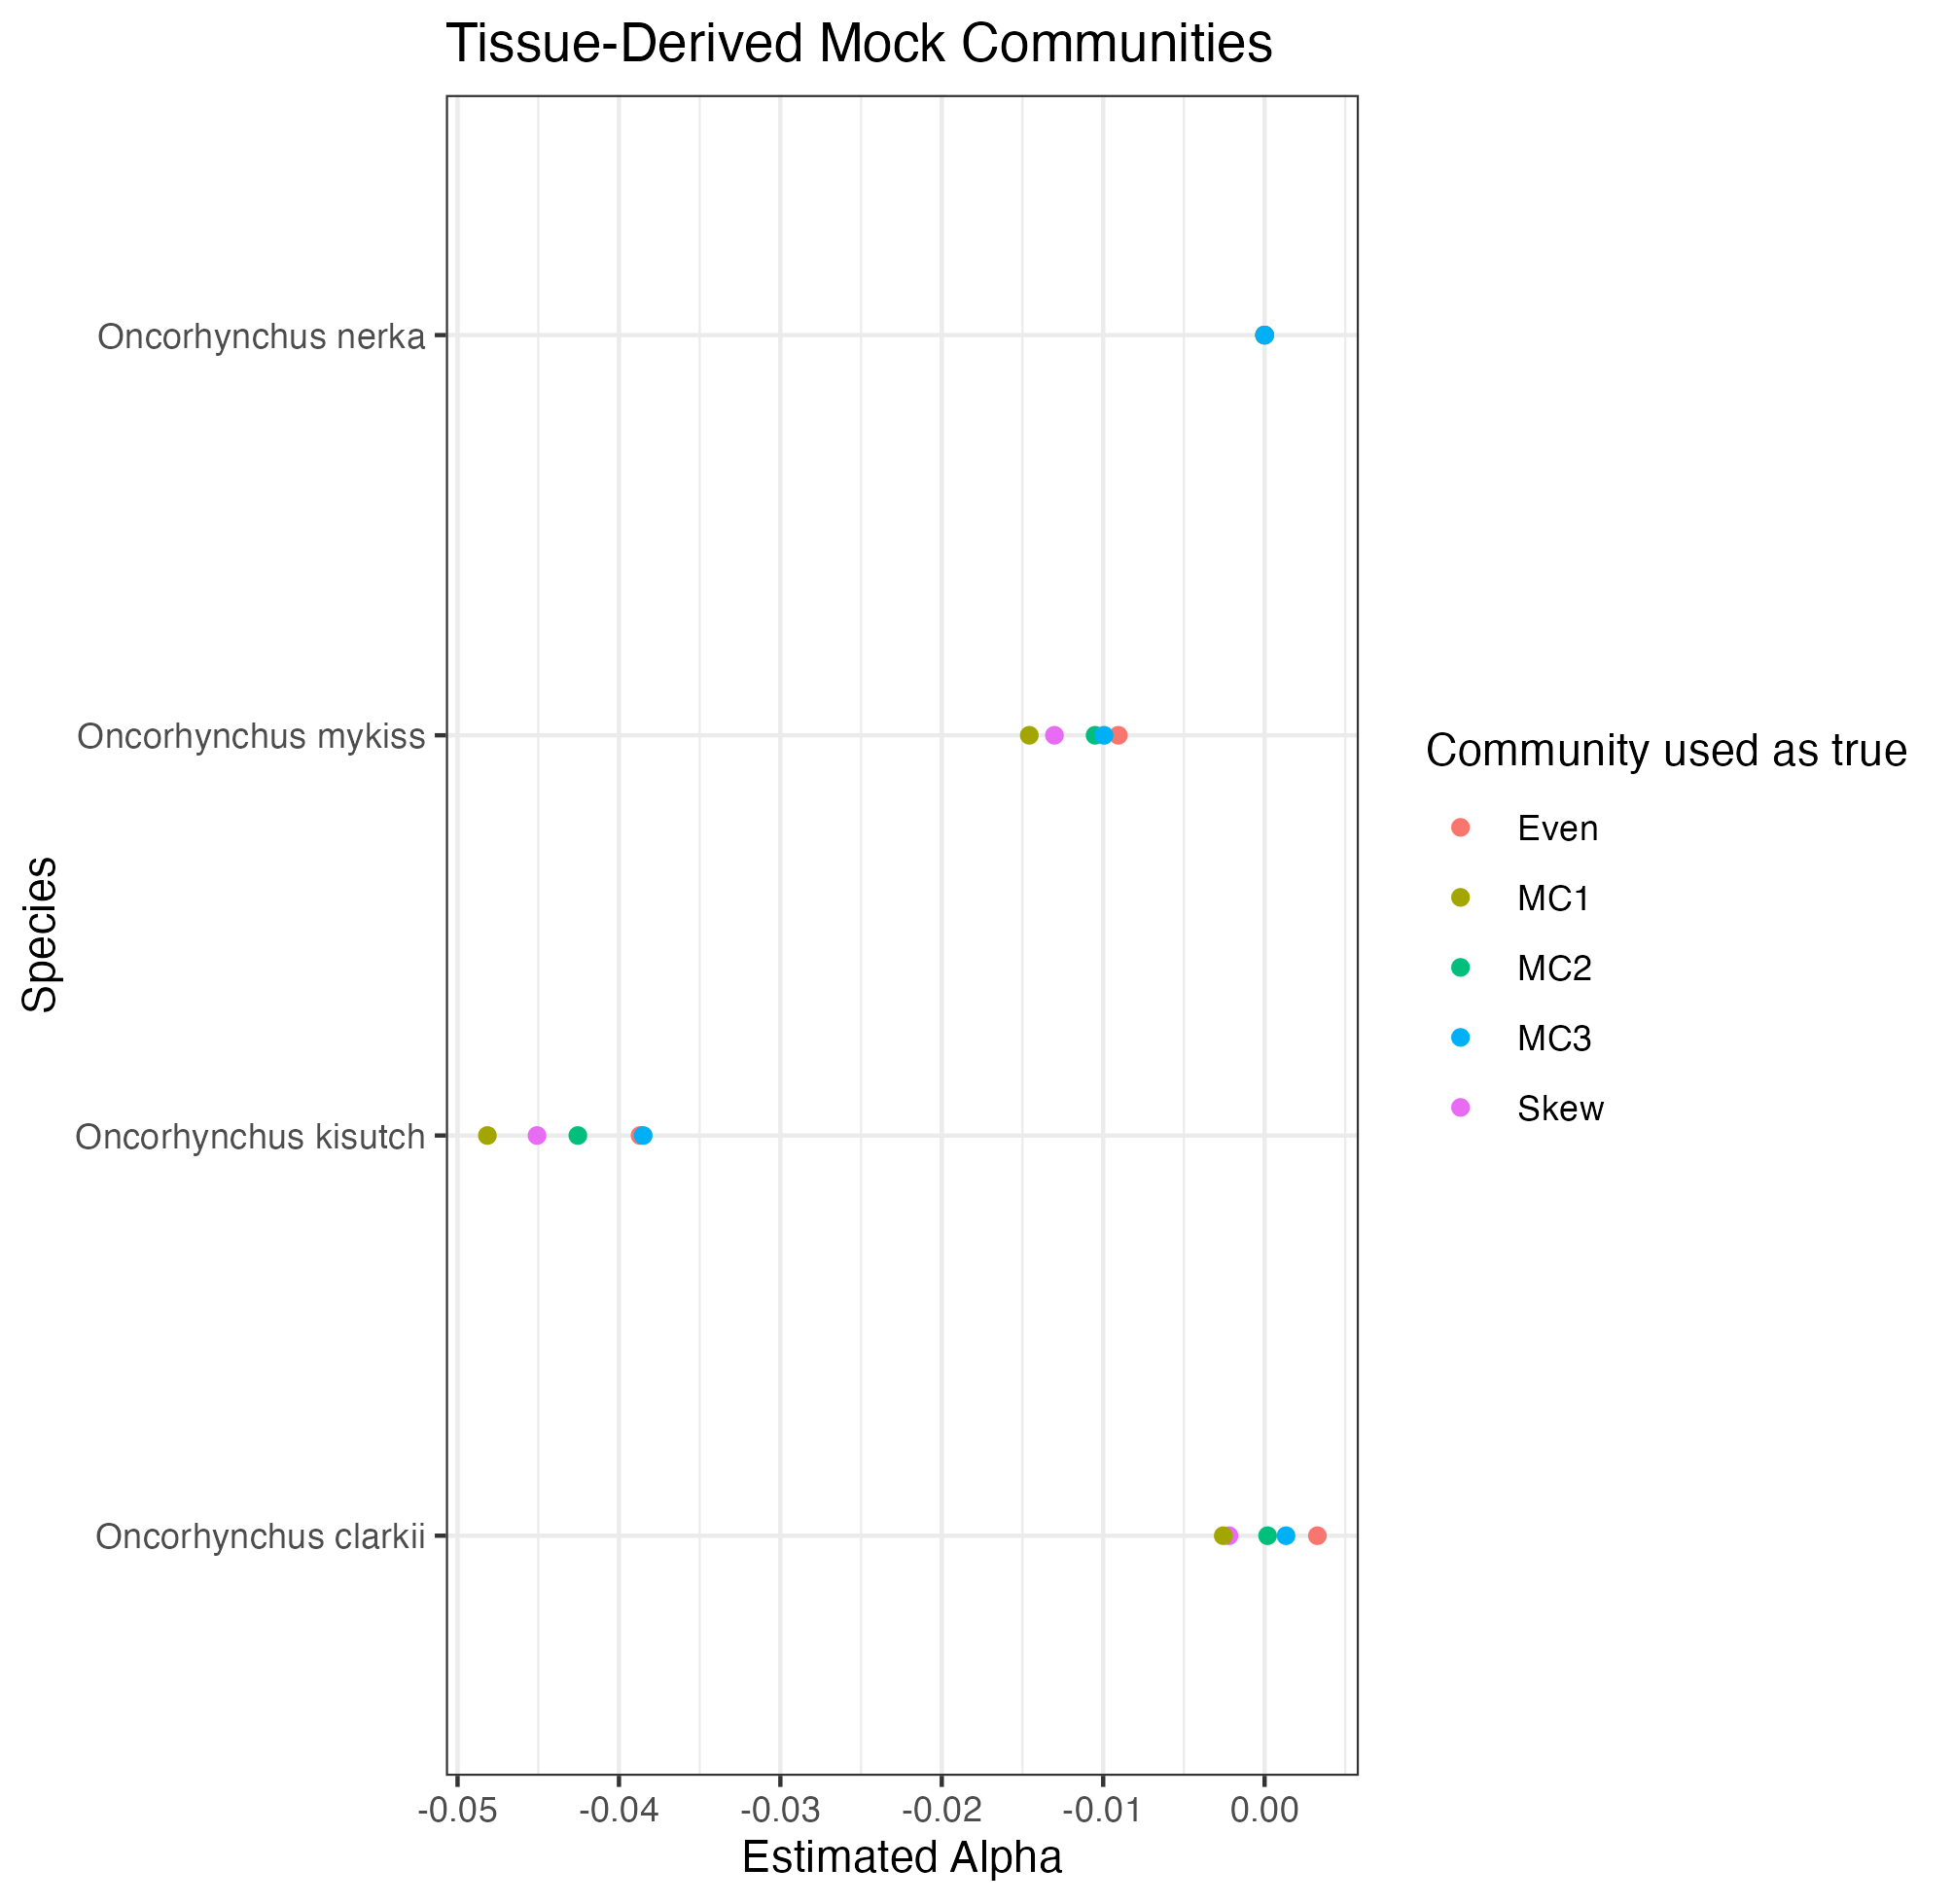
\includegraphics{../Output/SupplementalFigures/mock_internal_calibration_compare_alphas.png}
\caption{Estimated alpha values of salmonid species with different
calibrations of the mock communities. Each color represents a different
subset of mock community data treated as `true' to calibrate the
remainder of the mock community data.}
\end{figure}

We can then use the mock communities to correct the data from the MiSeq
(Supplementary Figure 9) to account for the different alpha values
(Supplementary Figure 8). The corrected results are shown in the main
text as Figure 3.

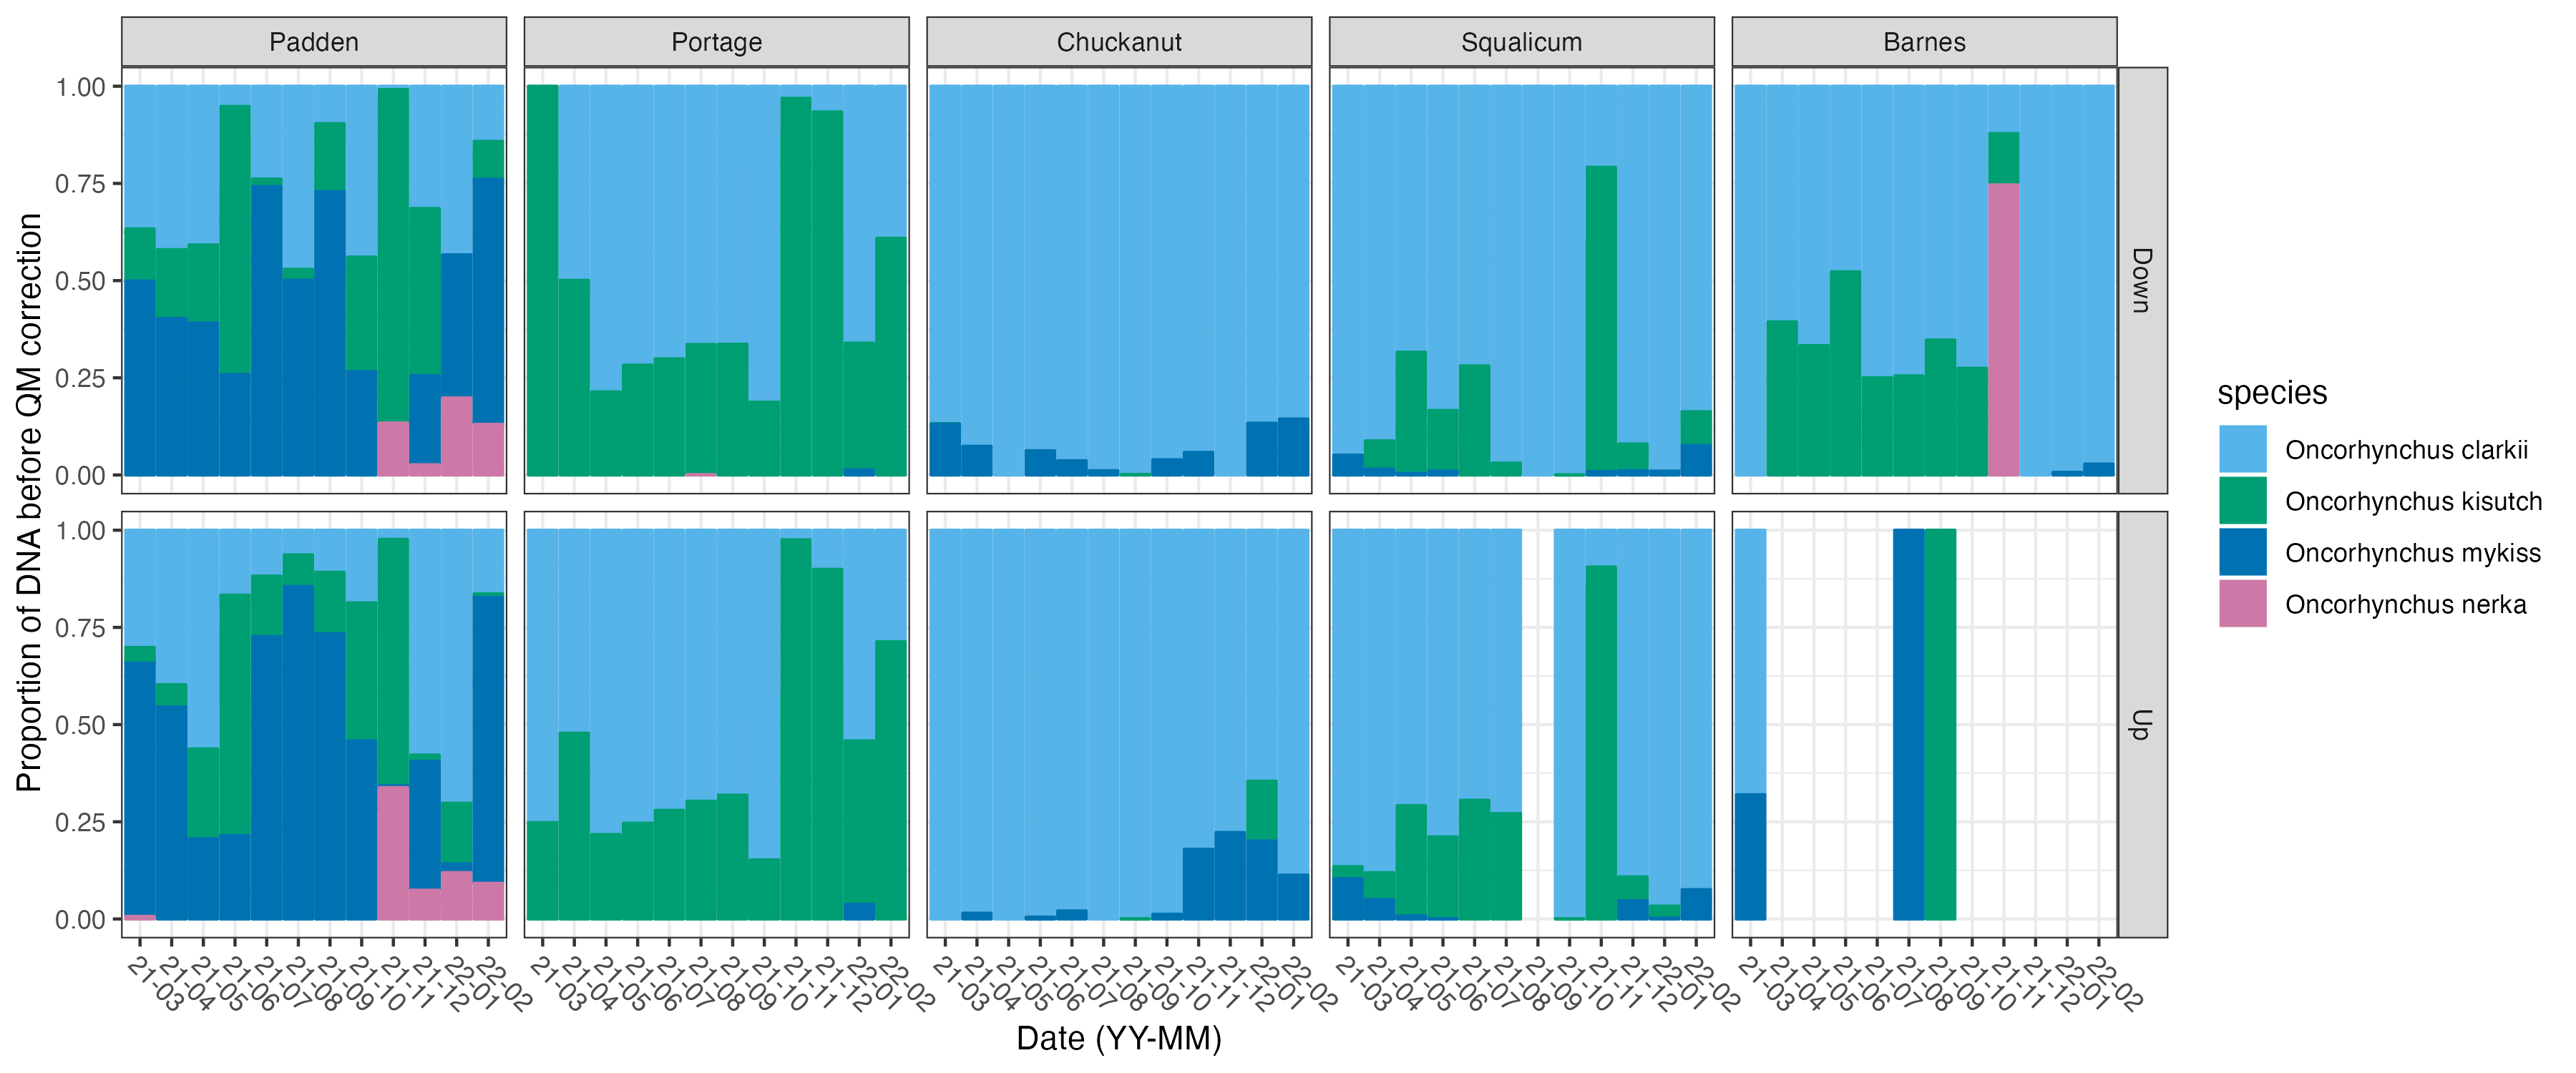
\includegraphics{../Output/SupplementalFigures/20221123_proportions_before_qm.png}
\#\# Effects of culverts In the main text, we show the effect of
culverts averaged over creeks and species. Here, we show them separate
(Supplementary Figure 10). The y-axis scale changes for each creek,
demonstrating that some culverts have a larger effect on the difference
between upstream and downstream than others. Namely, \emph{O. kisutch}
in Chuckanut Creek sees the largest percent difference. There also seems
to be a slight effect of season on the culverts, where summer months
often have the most highest difference between upstream and downstream
(i.e., higher eDNA concentrations upstream).

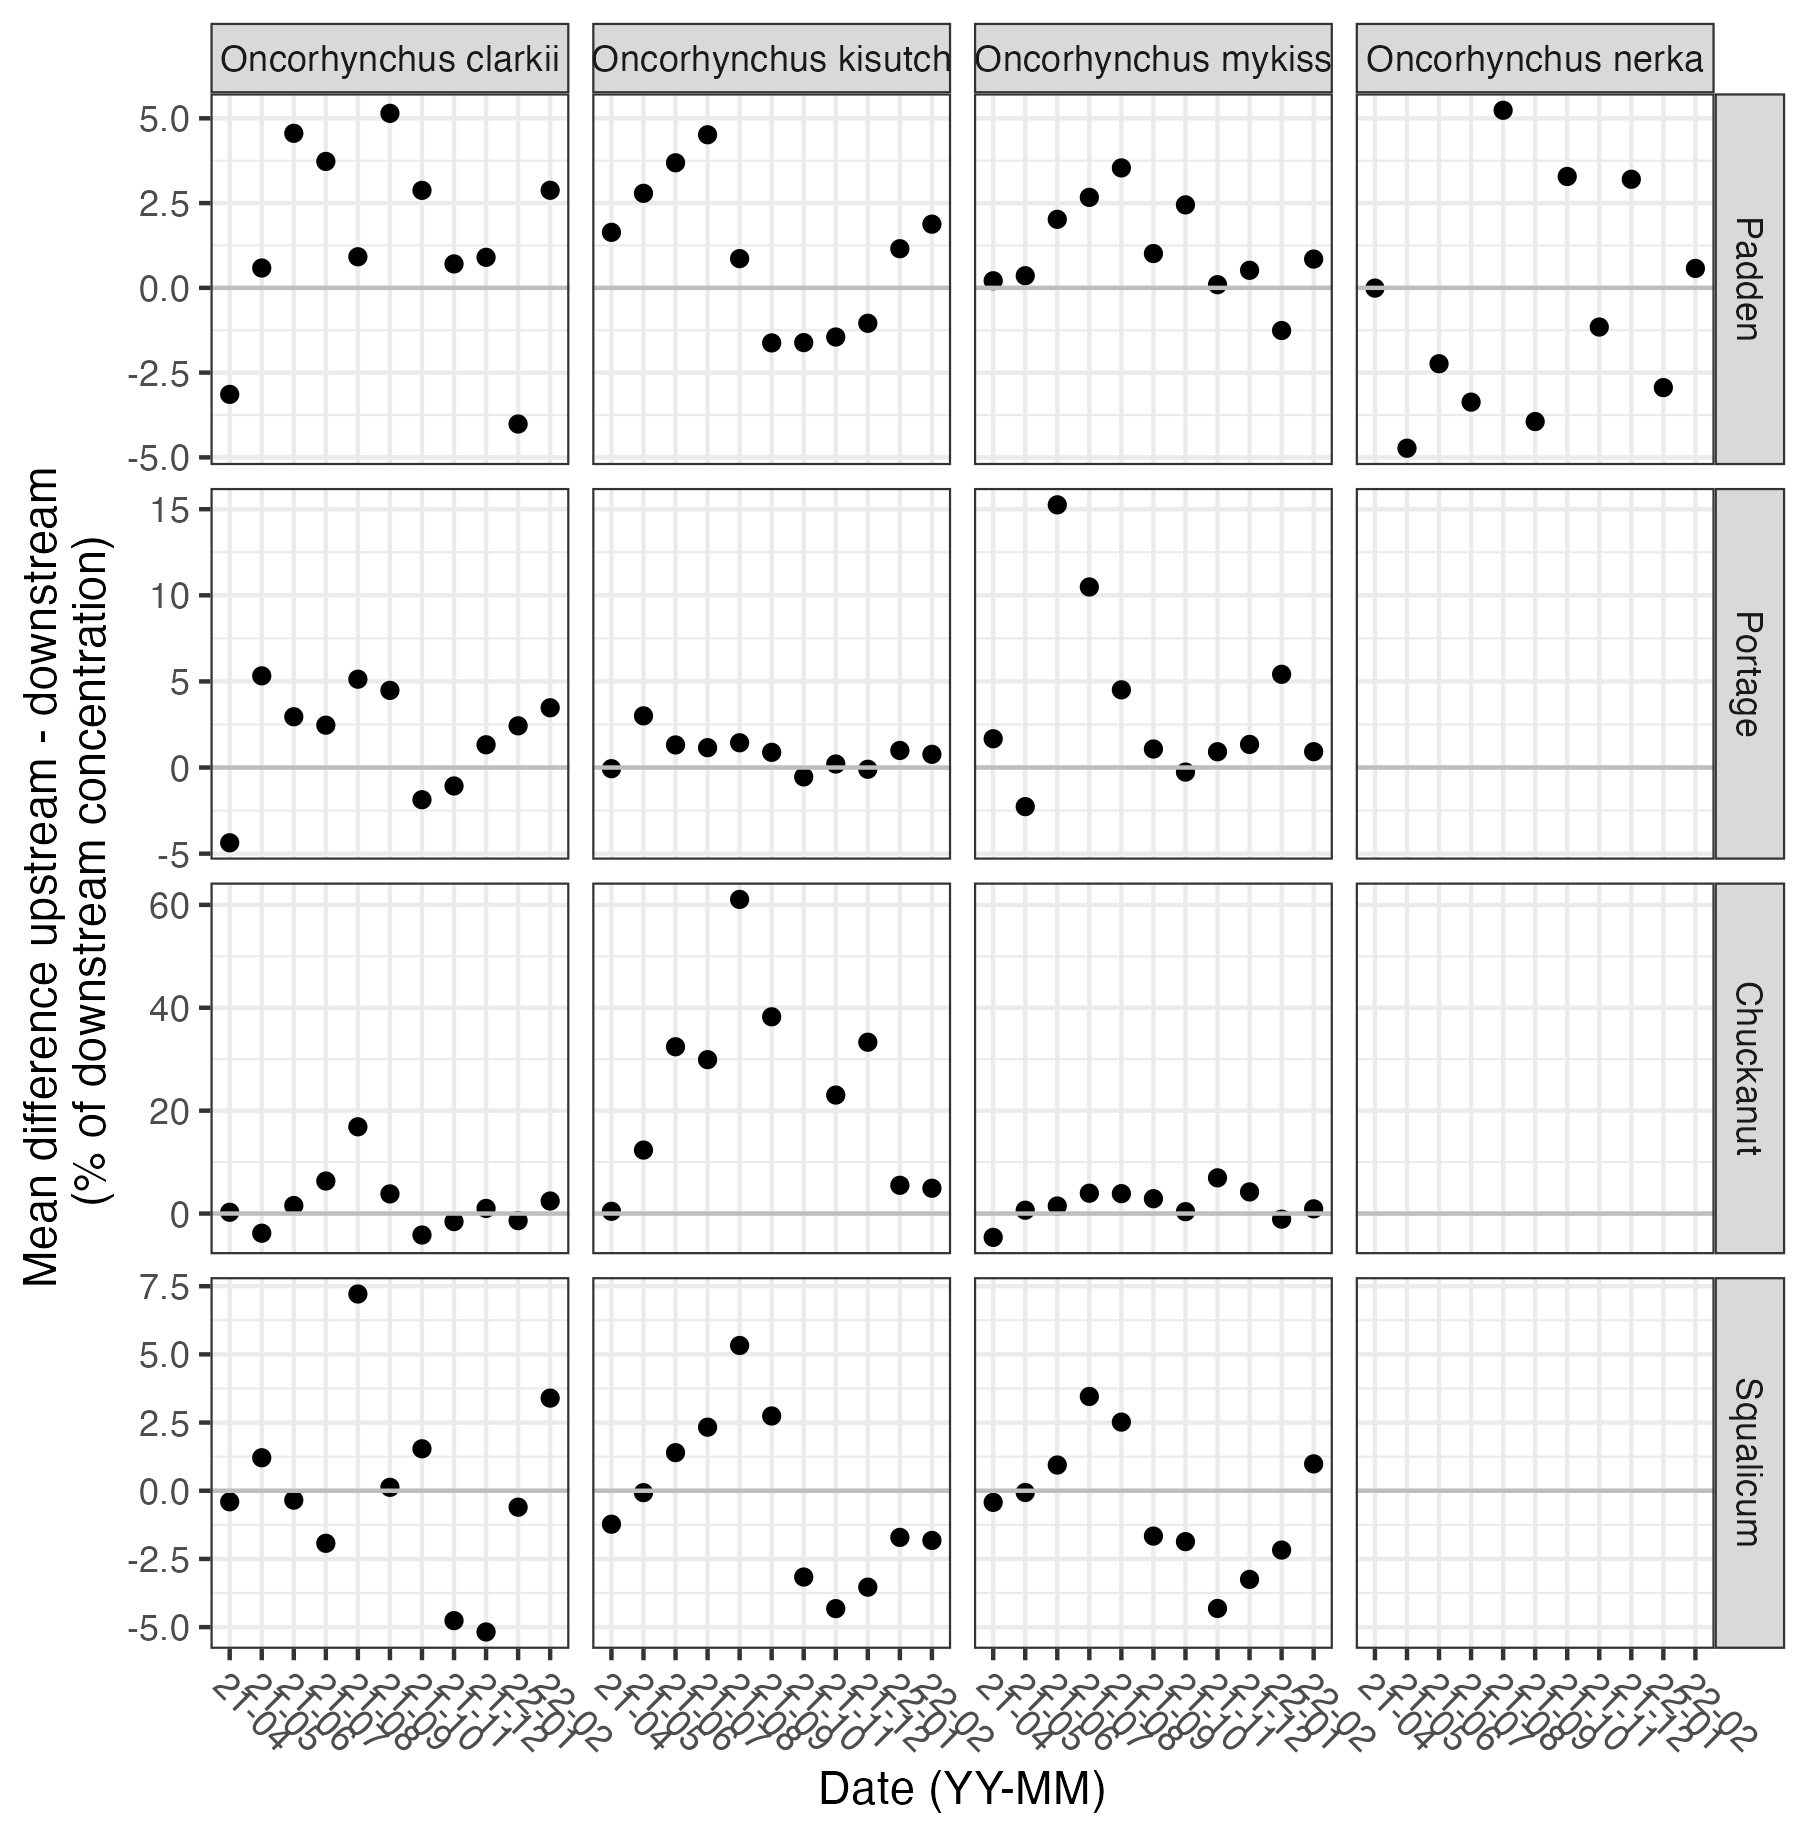
\includegraphics{../Output/SupplementalFigures/20221129_culvert_effect_creek_species_flowcorrected.png}
\#\# References

\hypertarget{refs}{}
\begin{CSLReferences}{1}{0}
\leavevmode\vadjust pre{\hypertarget{ref-callahan2016a}{}}%
Callahan, Benjamin J, Paul J McMurdie, Michael J Rosen, Andrew W Han,
Amy Jo A Johnson, and Susan P Holmes. 2016. {``DADA2: High Resolution
Sample Inference from Illumina Amplicon Data.''} \emph{Nature Methods}
13 (7): 581--83. \url{https://doi.org/10.1038/nmeth.3869}.

\leavevmode\vadjust pre{\hypertarget{ref-martin2011a}{}}%
Martin, Marcel. 2011. {``Cutadapt Removes Adapter Sequences from
High-Throughput Sequencing Reads.''} \emph{EMBnet.journal} 17 (1): 10.
\url{https://doi.org/10.14806/ej.17.1.200}.

\leavevmode\vadjust pre{\hypertarget{ref-thomas2018a}{}}%
Thomas, Austen C, Jesse Howard, Phong L Nguyen, Tracie A Seimon, and
Caren S Goldberg. 2018. {``ANDe {\texttrademark}: A Fully Integrated
Environmental DNA Sampling System.''} \emph{Methods in Ecology and
Evolution} 9 (6): 13791385.

\leavevmode\vadjust pre{\hypertarget{ref-thomas2019}{}}%
Thomas, Austen C., Phong L. Nguyen, Jesse Howard, and Caren S. Goldberg.
2019. {``A Self-Preserving, Partially Biodegradable eDNA Filter.''}
\emph{Methods in Ecology and Evolution} 10 (8): 1136--41.
\url{https://doi.org/10.1111/2041-210X.13212}.

\leavevmode\vadjust pre{\hypertarget{ref-wilkinson2018}{}}%
Wilkinson, Shaun P, Simon K Davy, Michael Bunce, and Michael Stat. 2018.
{``Taxonomic Identification of Environmental DNA with Informatic
Sequence Classification Trees.''}
\url{https://doi.org/10.7287/peerj.preprints.26812v1}.

\end{CSLReferences}

\end{document}
